\documentclass[
	a4paper,
	oneside,
	BCOR = 10mm,
	DIV = 12,
	12pt,
	headings = normal,
]{scrartcl}

%%% Length calculations
\usepackage{calc}
%%%

%%% Support for color
\usepackage{xcolor}
\definecolor{lightblue}{HTML}{03A9F4}
\definecolor{red}{HTML}{F44336}
%%%

%%% Including graphics
\usepackage{graphicx}
%%%

%%% Font selection
\usepackage{fontspec}

\setromanfont{STIX Two Text}[
	SmallCapsFeatures = {LetterSpace = 8},
]

\setsansfont{IBM Plex Sans}[
	Scale = MatchUppercase,
]

\setmonofont{IBM Plex Mono}[
	Scale = MatchUppercase,
]
%%%

%%% Math typesetting
\usepackage{amsmath}

\usepackage{unicode-math}
\setmathfont{STIX Two Math}

\usepackage{IEEEtrantools}
%%%

%%% List settings
\usepackage{enumitem}
\setlist[enumerate]{
	label*      = {\arabic*.},
	left        = \parindent,
	topsep      = 0\baselineskip,
	parsep      = 0\baselineskip,
	noitemsep, % override itemsep
}
% List settings for levels 2–4
\setlist[enumerate, 2, 3, 4]{
	label*      = {\arabic*.},
	left        = 0em,
	topsep      = 0\baselineskip,
	parsep      = 0\baselineskip,
	noitemsep, % override itemsep
}

\setlist[itemize]{
	label*      = {—},
	left        = \parindent,
	topsep      = 0\baselineskip,
	parsep      = 0\baselineskip,
	itemsep     = 1\baselineskip,
	noitemsep, % override itemsep
}

\setlist[description]{
	font        = {\rmfamily\upshape\bfseries},
	topsep      = 1\baselineskip,
	parsep      = 0\baselineskip,
	itemsep     = 0\baselineskip,
}

%%%

%%% Structural elements typesetting
\setkomafont{pagenumber}{\rmfamily\upshape}
\setkomafont{disposition}{\rmfamily\bfseries}

% Sectioning
\RedeclareSectionCommand[
	beforeskip = -1\baselineskip,
	afterskip  = 1\baselineskip,
	font       = {\normalsize\bfseries\scshape},
]{section}

\RedeclareSectionCommand[
	beforeskip = -1\baselineskip,
	afterskip  = 1\baselineskip,
	font       = {\normalsize\bfseries\itshape},
]{subsection}

\RedeclareSectionCommand[
	beforeskip = -1\baselineskip,
	afterskip  = 1\baselineskip,
	font       = {\normalsize\bfseries},
]{subsubsection}

\RedeclareSectionCommand[
	beforeskip = -1\baselineskip,
	afterskip  = -0.5em,
	font       = {\normalsize\mdseries\scshape\addfontfeatures{Letters = {UppercaseSmallCaps}}},
]{paragraph}
%%%

%%% Typographic enhancements
\usepackage{microtype}
%%%

%%% Language-specific settings
\usepackage{polyglossia}
\setmainlanguage{ukrainian}
\setotherlanguages{english}
%%%

%%% Captions
\usepackage{caption}
\usepackage{subcaption}

%\DeclareCaptionLabelFormat{closing}{#2)}
%\captionsetup[subtable]{labelformat = closing}

%\captionsetup[subfigure]{labelformat = closing}

\captionsetup[table]{
	aboveskip = 0\baselineskip,
	belowskip = 0\baselineskip,
}

\captionsetup[figure]{
	aboveskip = 1\baselineskip,
	belowskip = 0\baselineskip,
}

\captionsetup[subfigure]{
	labelformat = simple,
	labelformat = brace,
	% justification = RaggedRight,
	% singlelinecheck = false,
}
%%%

%%% Hyphenated ragged typesetting
\usepackage{ragged2e}
%%%

%%% Table typesetting
\usepackage{booktabs}
\usepackage{longtable}

\usepackage{multirow}

\usepackage{array}
\newcolumntype{v}[1]{>{\RaggedRight\arraybackslash\hspace{0pt}}p{#1}}
\newcolumntype{b}[1]{>{\Centering\arraybackslash\hspace{0pt}}p{#1}}
\newcolumntype{n}[1]{>{\RaggedLeft\arraybackslash\hspace{0pt}}p{#1}}
%%%

%%% Drawing
\usepackage{tikz}
\usepackage{tikzscale}
\usetikzlibrary{positioning}
\usetikzlibrary{arrows.meta} % Stealth arrow tips
%%%

%%% SI units typesetting
\usepackage{siunitx}
\sisetup{
	output-decimal-marker = {,},
	exponent-product      = {\cdot},
	inter-unit-product    = \ensuremath{{} \cdot {}},
	per-mode              = symbol,
}
%%%

% Code Highlighting
\usepackage{minted}
\setmintedinline{
	style = bw,
	breaklines,
}

\newminted[bashterm]{text}{%
	autogobble,%
	breaklines,%
	style=bw,%
}

\newminted[codegeneric]{text}{%
	autogobble,%
	style=bw,%
	breaklines,%
	fontsize=\small,%
}

\newmintinline{bash}{%
}

\newmintinline[minttext]{text}{%
	breaklines,%
	breakanywhere,%
}

%%% Framing code listings
\usepackage{tcolorbox}
\tcbuselibrary{breakable}
\tcbuselibrary{minted}
\tcbuselibrary{skins}

% Text file listing
\newtcblisting[
	auto counter,
	list inside,
	number within = section,
]{listingplaintext}[3][]{%
	minted language = text,
	minted style    = bw,
	minted options  = {
		autogobble,
		linenos,
		tabsize = 4,
		breaklines,
		breakanywhere,
		fontsize = \footnotesize,
	},
	empty,
	sharp corners,
	coltitle = black,
	borderline horizontal = {1pt}{0pt}{black},
	titlerule = {0.5pt},
	titlerule style = {
		black,
	},
	toptitle = 0.3em,
	bottomtitle = 0.3em,
	before skip      = \intextsep,
	after  skip      = \intextsep,
	title            = {Лістинг \thetcbcounter: #2},
	list entry       = {\protect\numberline{\thetcbcounter}#2},
	left = 0em,
	right = 0em,
	%
	listing only,
	breakable,
	%
	label = {#3},%
}

\newtcblisting[
	use counter from = listingplaintext,
	list inside,
	number within = section,
]{listingpython}[3][]{%
	minted language = python,
	minted style    = bw,
	minted options  = {
		autogobble,
		linenos,
		tabsize = 4,
		breaklines,
		breakanywhere,
		fontsize = \footnotesize,
	},
	empty,
	sharp corners,
	coltitle = black,
	borderline horizontal = {1pt}{0pt}{black},
	titlerule = {0.5pt},
	titlerule style = {
		black,
	},
	toptitle = 0.3em,
	bottomtitle = 0.3em,
	before skip      = \intextsep,
	after  skip      = \intextsep,
	title            = {Лістинг \thetcbcounter: #2},
	list entry       = {\protect\numberline{\thetcbcounter}#2},
	left = 0em,
	right = 0em,
	%
	listing only,
	breakable,
	%
	label = {#3},
	%
	#1%
}

\newtcbinputlisting[
	use counter from = listingplaintext,
	list inside,
	number within = section
]{\inputpython}[4][]{%
	minted language = python,
	minted style    = bw,
	minted options  = {
		autogobble,
		linenos,
		tabsize = 4,
		breaklines,
		breakanywhere,
		fontsize = \footnotesize,
	},
	empty,
	sharp corners,
	coltitle = black,
	borderline horizontal = {1pt}{0pt}{black},
	titlerule = {0.5pt},
	titlerule style = {
		black,
	},
	toptitle = 0.3em,
	bottomtitle = 0.3em,
	before skip      = \intextsep,
	after  skip      = \intextsep,
	title            = {Лістинг \thetcbcounter: #3},
	list entry       = {\protect\numberline{\thetcbcounter}#3},
	left = 0em,
	right = 0em,
	%
	listing file={#2},
	listing only,
	breakable,
	%
	label = {#4}
}

% Linux command-line listing
\newtcblisting{linuxterm}%
{%
	% Syntax highlighing options
	listing only,%
	minted language = bash,%
	minted options={%
		autogobble,%
		linenos%
	},%
	% Presentation options
	empty,%
	%% Margins
	sharp corners,%
	toptitle = 0.0em,%
	bottomtitle = 0.0em,%
	left = 0em,%
	right = 0em,%
	before skip = \intextsep,%
	after skip = \intextsep,%
}

\newtcblisting{linuxtermout}%
{%
	% Syntax highlighing options
	listing only,%
	minted language = text,%
	minted options={%
		autogobble,%
		linenos%
	},%
	% Presentation options
	empty,%
	%% Margins
	sharp corners,%
	toptitle = 0.0em,%
	bottomtitle = 0.0em,%
	left = 0em,%
	right = 0em,%
	before skip = \intextsep,%
	after skip = \intextsep,%
}

% Dockerfile listings
\newtcblisting[
	use counter from = listingplaintext,
	list inside,
	number within = section,
]{listingdocker}[3][]{%
	minted language = dockerfile,
	minted style    = bw,
	minted options  = {
		autogobble,%
		linenos,
		tabsize = 4,
		breaklines,
		breakanywhere,
		fontsize = \footnotesize,
	},
	empty,
	sharp corners,
	coltitle = black,
	borderline horizontal = {1pt}{0pt}{black},
	titlerule = {0.5pt},
	titlerule style = {
		black,
	},
	toptitle = 0.3em,
	bottomtitle = 0.3em,
	before skip      = \intextsep,
	after  skip      = \intextsep,
	title            = {Лістинг \thetcbcounter: #2},
	list entry       = {\protect\numberline{\thetcbcounter}#2},
	left = 0em,
	right = 0em,
	%
	listing only,
	breakable,
	%
	label = {#3},%
}

% Docker Compose listings
\newtcblisting[
	use counter from = listingplaintext,
	list inside,
	number within = section,
]{listingdockercompose}[3][]{%
	minted language = yaml,
	minted style    = bw,
	minted options  = {
		autogobble,%
		linenos,
		tabsize = 4,
		breaklines,
		breakanywhere,
		fontsize = \footnotesize,
	},
	empty,
	sharp corners,
	coltitle = black,
	borderline horizontal = {1pt}{0pt}{black},
	titlerule = {0.5pt},
	titlerule style = {
		black,
	},
	toptitle = 0.3em,
	bottomtitle = 0.3em,
	before skip      = \intextsep,
	after  skip      = \intextsep,
	title            = {Лістинг \thetcbcounter: #2},
	list entry       = {\protect\numberline{\thetcbcounter}#2},
	left = 0em,
	right = 0em,
	%
	listing only,
	breakable,
	%
	label = {#3},%
}


% Customize minted line numbers
\renewcommand{\theFancyVerbLine}{\ttfamily\scriptsize\arabic{FancyVerbLine}}

%%%

%%% Typeset menus and keys
\usepackage{menukeys}[
	os=win,
]
%%%

%%% Links and hyperreferences
\usepackage{hyperref}
\hypersetup{
	bookmarksnumbered = true,
	colorlinks      = false,
	linkbordercolor = red,
	urlbordercolor  = lightblue,
	pdfborderstyle  = {/S/U/W 1.5},
}
%%%

%%% Length adjustment

% Set baselineskip, default is 14.5 pt
\linespread{1.068966} % ~15.5 pt
\setlength{\emergencystretch}{1em}
\setlength{\parindent}{1.5em}
\newlength{\gridunitwidth}
\setlength{\gridunitwidth}{\textwidth / 12}
%%%

%%% Custom commands
\newcommand{\allcaps}[1]{%
	{%
		\addfontfeatures{%
			Letters = UppercaseSmallCaps,
			LetterSpace = 8,%
		}%
		#1%
	}%
}
\newcommand{\filename}[1]{\texttt{#1}}
\newcommand{\progname}[1]{\texttt{#1}}
\newcommand{\commandname}[1]{\texttt{#1}}
\newcommand{\modulename}[1]{\texttt{#1}}
\newcommand{\transeng}[1]{{англ.}~\textit{\textenglish{#1}}}
%%%

%%% Custom math commands
\newcommand{\longvar}[1]{\mathit{#1}}
%%%

\begin{document}

\begin{titlepage}
		\begin{center}
			Міністерство освіти і~науки України\\
			Національний авіаційний університет\\
			Факультет кібербезпеки, комп'ютерної та~програмної інженерії\\
			Кафедра комп'ютеризованих систем управління

			\vspace{\fill}
				Лабораторна робота №~1.4\\
				з~дисципліни «Захист інформації в~комп'ютерних системах»\\
				на~тему «Керування віддаленим комп'ютером»

			\vspace{\fill}

			\begin{flushright}
				Виконав:\\
				студент \allcaps{ФККПІ}\\
				групи \allcaps{СП}-425\\
				Рабін І.\,Р.\\
				Перевірила:\\
				Супрун О.\,М.
			\end{flushright}

			Київ 2019
		\end{center}
	\end{titlepage}

	\section{Мета роботи}
		Ознайомитись з~можливостями керування віддаленим комп'ютером.

	\section{Завдання роботи}
		Ознайомитись із~програмними засобами віддаленого адміністрування та~відповідними протоколами; встановити програми віддаленого адміністрування та~навчитись їх~використовувати.

	\section{Хід~роботи}
		\subsection{Програма~\textenglish{Teamviewer}}
			Готуємо дві~системи для~проведення лабораторної роботи. Для~цього встановлюємо на~них~програму~\textenglish{Teamviewer} і~запускаємо її. Перевіряємо можливість віддаленого керування. Для~цього після запуску обираємо вкладку «Віддалене керування», на~керуючій системі у~вікні~\textenglish{Teamviewer} вводимо \textenglish{\allcaps{ID}} і~пароль системи, якою треба керувати, і~натискаємо кнопку «Підключитись». В~результаті на~керуючій системі з'явиться вікно для~управління керованою системою~(рис.~\ref{fig:01-teamviewer-remote-ctl}).

			\begin{figure}[!htbp]
				\centering
				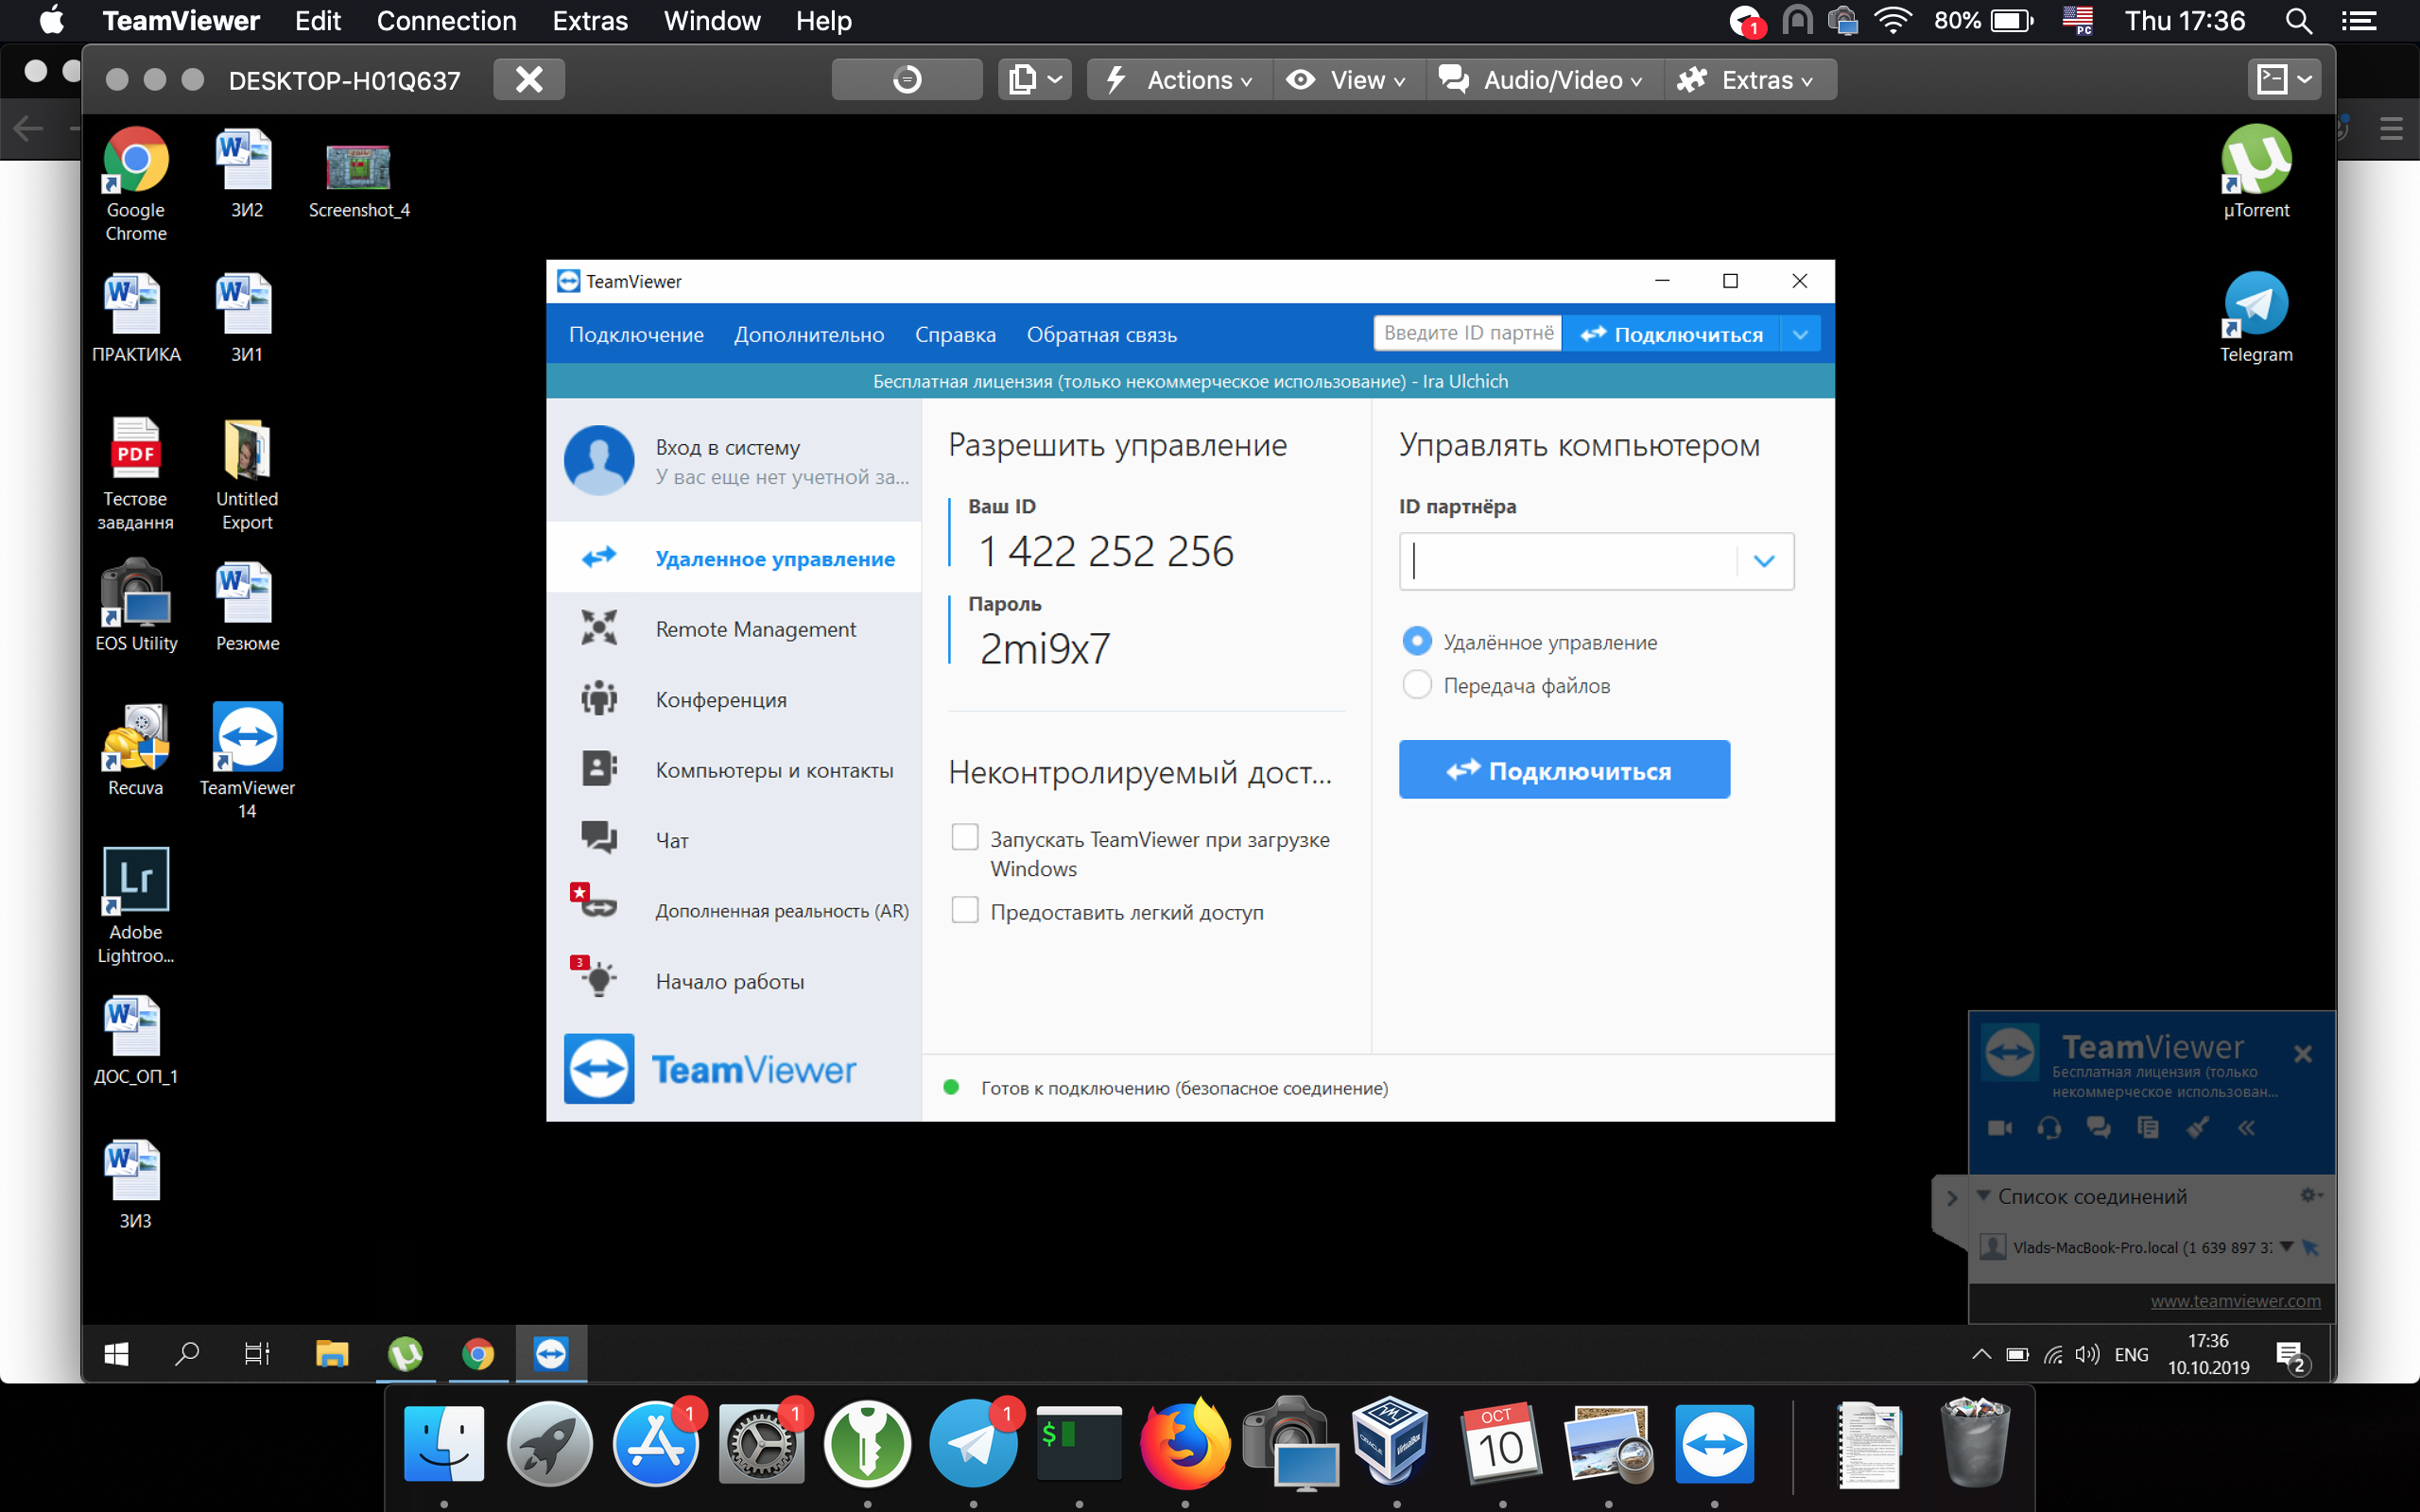
\includegraphics[width = 8\gridunitwidth]{./assets/p03-01.png}
				\caption{Програма~\textenglish{Teamviewer} на~керуючій системі: вікно управління керованою системою}
				\label{fig:01-teamviewer-remote-ctl}
			\end{figure}

			Тепер перевіряємо можливість проведення конференції. Для~цього на~керуючій системі відкриваємо вкладку «Конференція», у~підзаголовку «Розпочати конференцію» обираємо необхідний тип~конференції (презентація, відеоконференція чи~телефонна конференція) і~натискаємо на~відповідну іконку. В~результаті керуюча система розпочне конференцію, до~якої може підключитись керована. Коли керована система підключиться, вона бачитиме вміст екрану керуючої системи~(рис.~\ref{fig:02-teamviewer-meeting}).

			\begin{figure}[!htbp]
				\centering
				\begin{subfigure}[b]{8\gridunitwidth}
					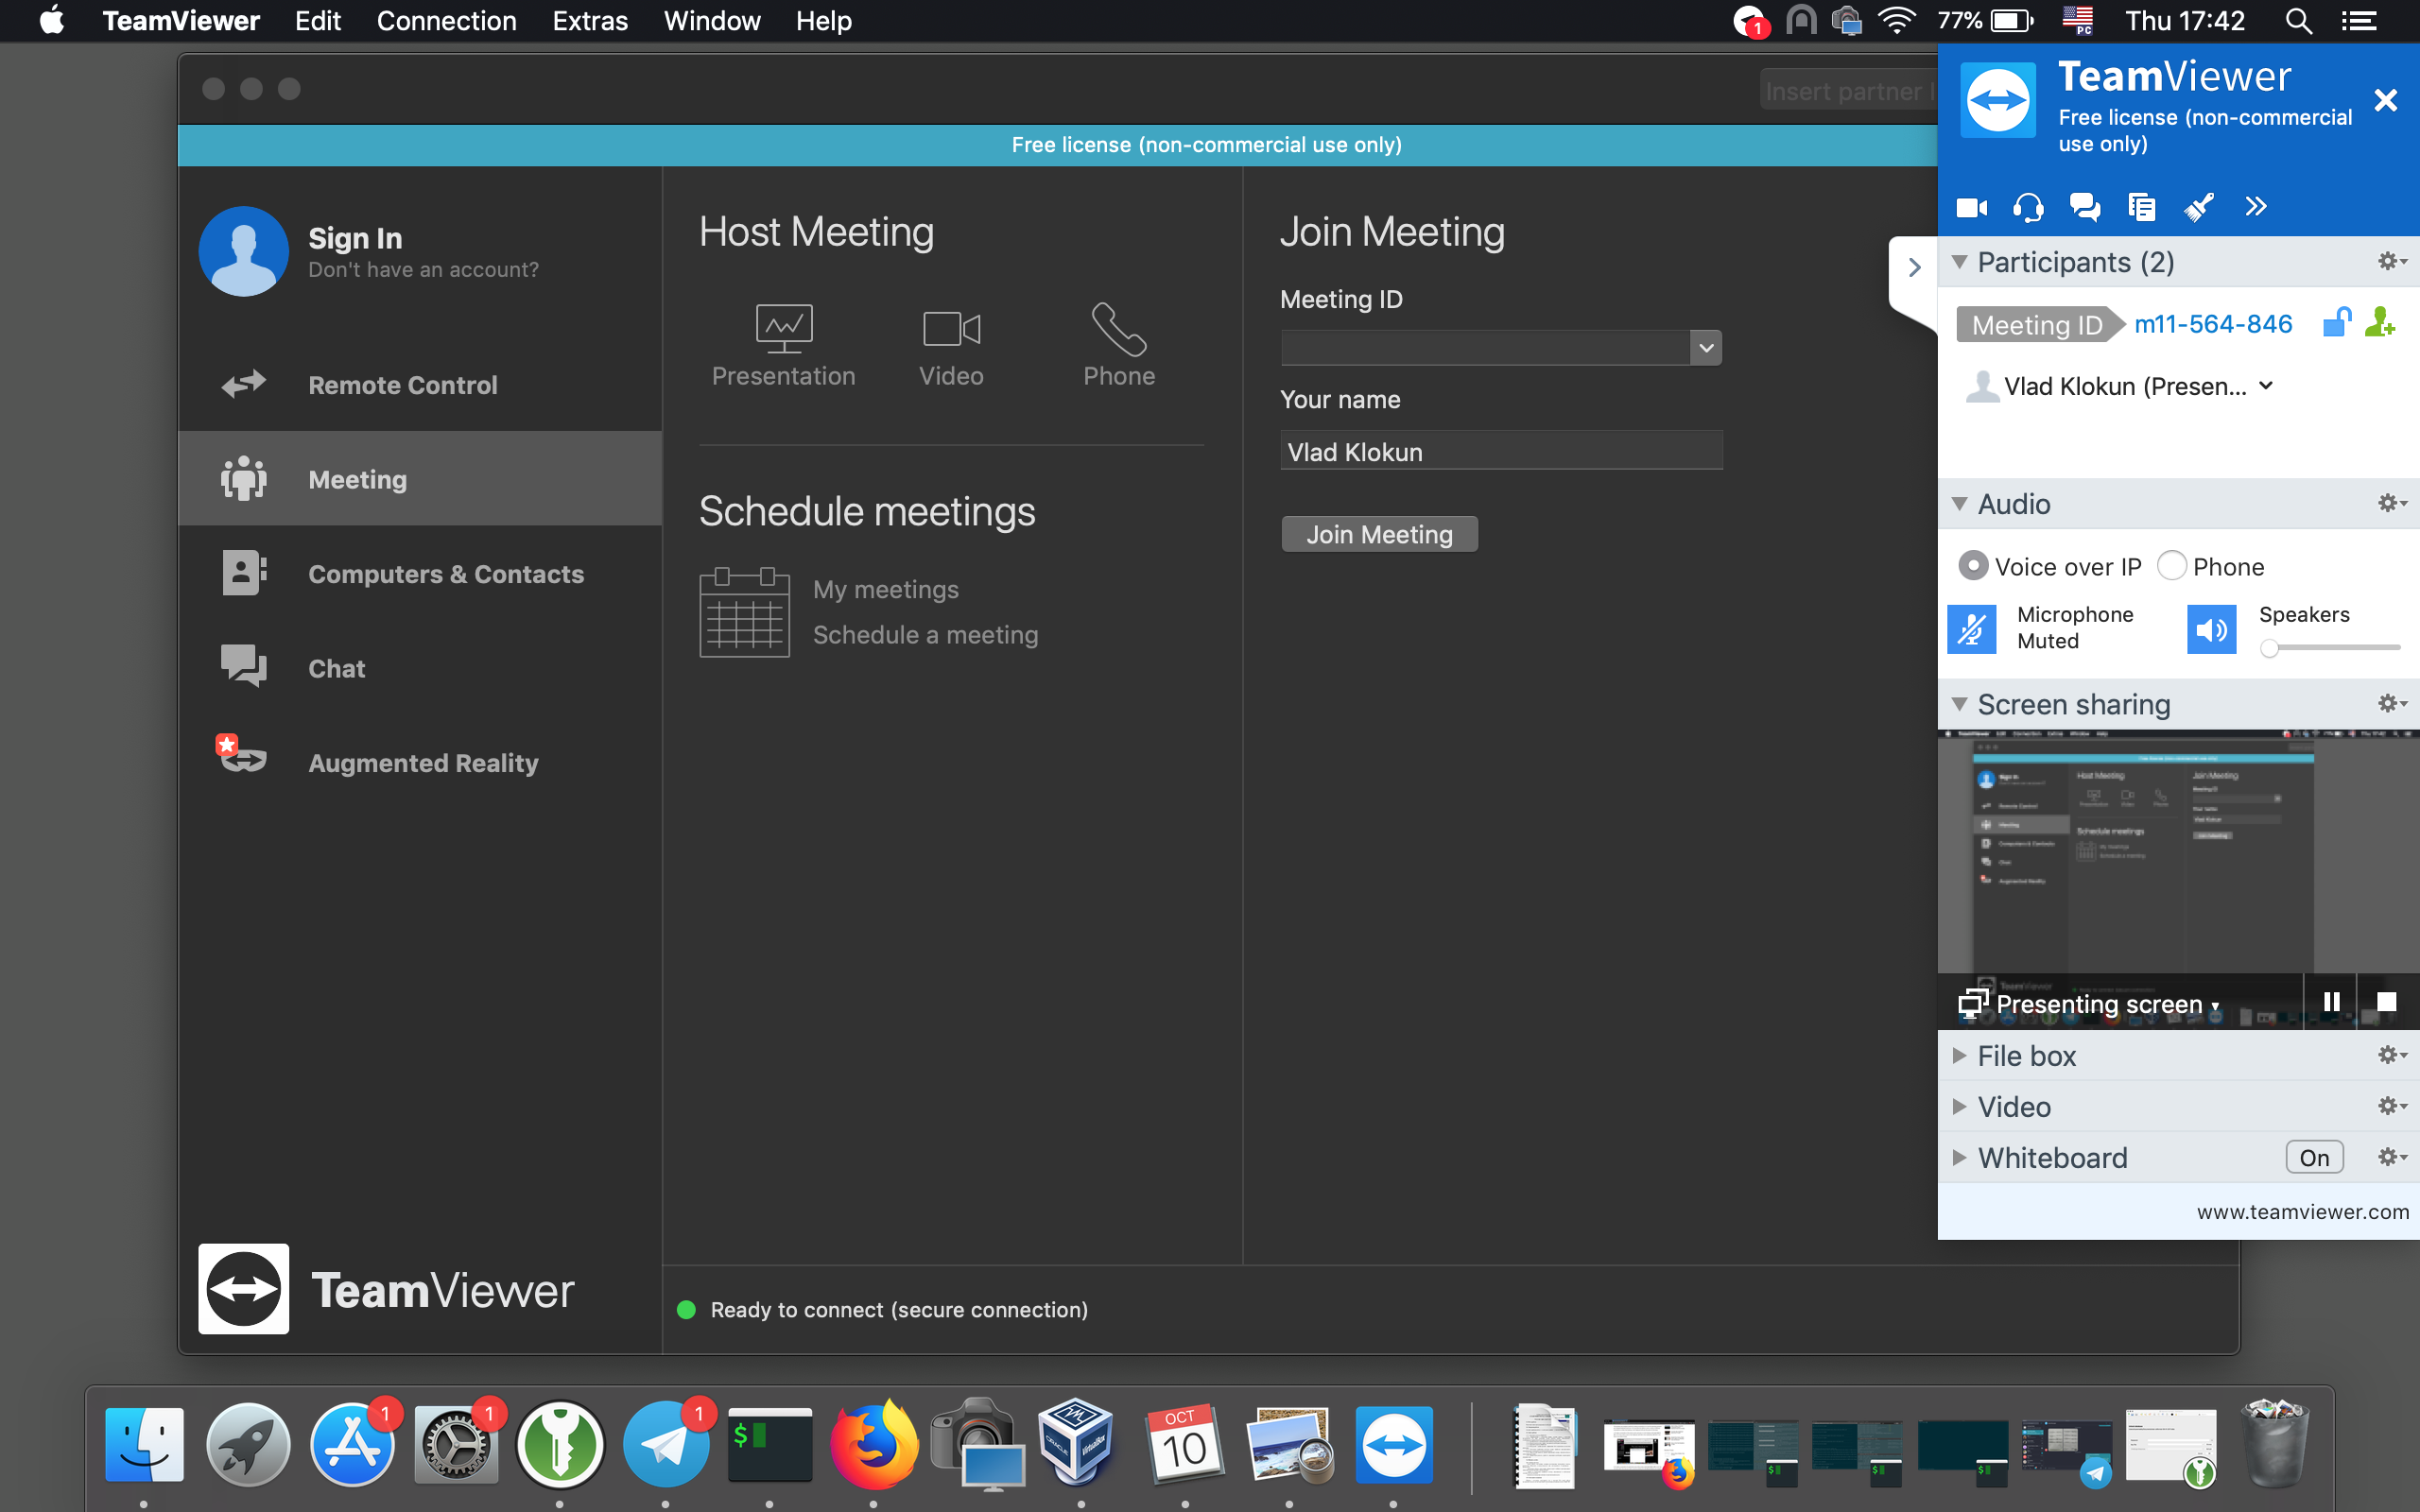
\includegraphics[width = \columnwidth]{./assets/p03-02.png}
					\caption{}
					\label{subfig:02-teamviewer-meeting-01}
				\end{subfigure}
				\begin{subfigure}[b]{8\gridunitwidth}
					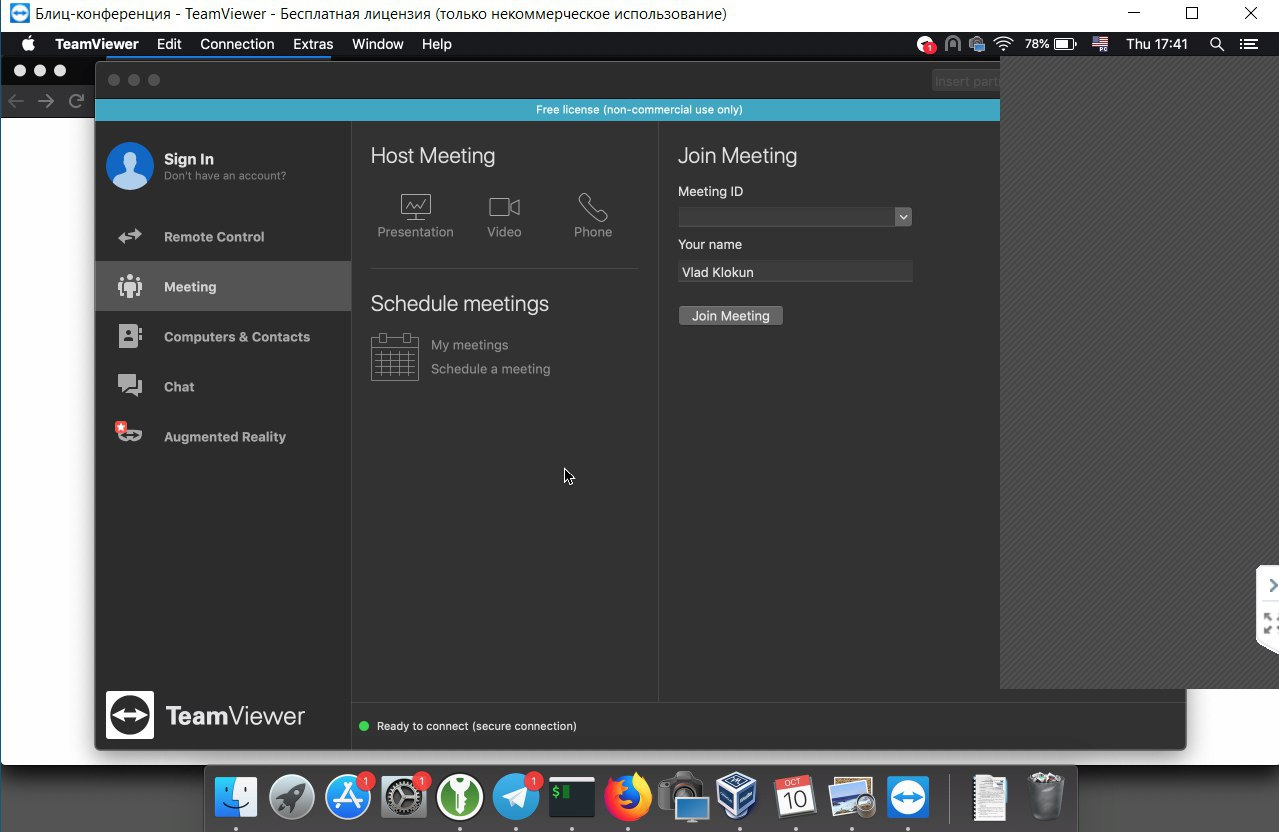
\includegraphics[width = \columnwidth]{./assets/p03-03.jpeg}
					\caption{}
					\label{subfig:02-teamviewer-meeting-02}
				\end{subfigure}
				\caption{Режим презентації в~\textenglish{Teamviewer}: \subref{subfig:02-teamviewer-meeting-01}~— екран керуючої системи після початку перезентації, \subref{subfig:02-teamviewer-meeting-02}~— вікно, в~якому транслюється презентація з~керуючої системи на~віддаленій}
				\label{fig:02-teamviewer-meeting}
			\end{figure}

			Перевіряємо можливість передачі файлів. Для~цього переходимо у~вкладку «Віддалене управління», вводимо дані керованої системи, обираємо варіант «передача файлів» і~натискаємо кнопку «Підключитись». В~результаті на~керуючій системі відкриється вікно вибору, які~файли передати, а~на~керованій~— повідомлення про~початок передачі файлів~(рис.~\ref{fig:03-teamviewer-file-transfer}).

			\begin{figure}[!htbp]
				\centering
				\begin{subfigure}[b]{8\gridunitwidth}
					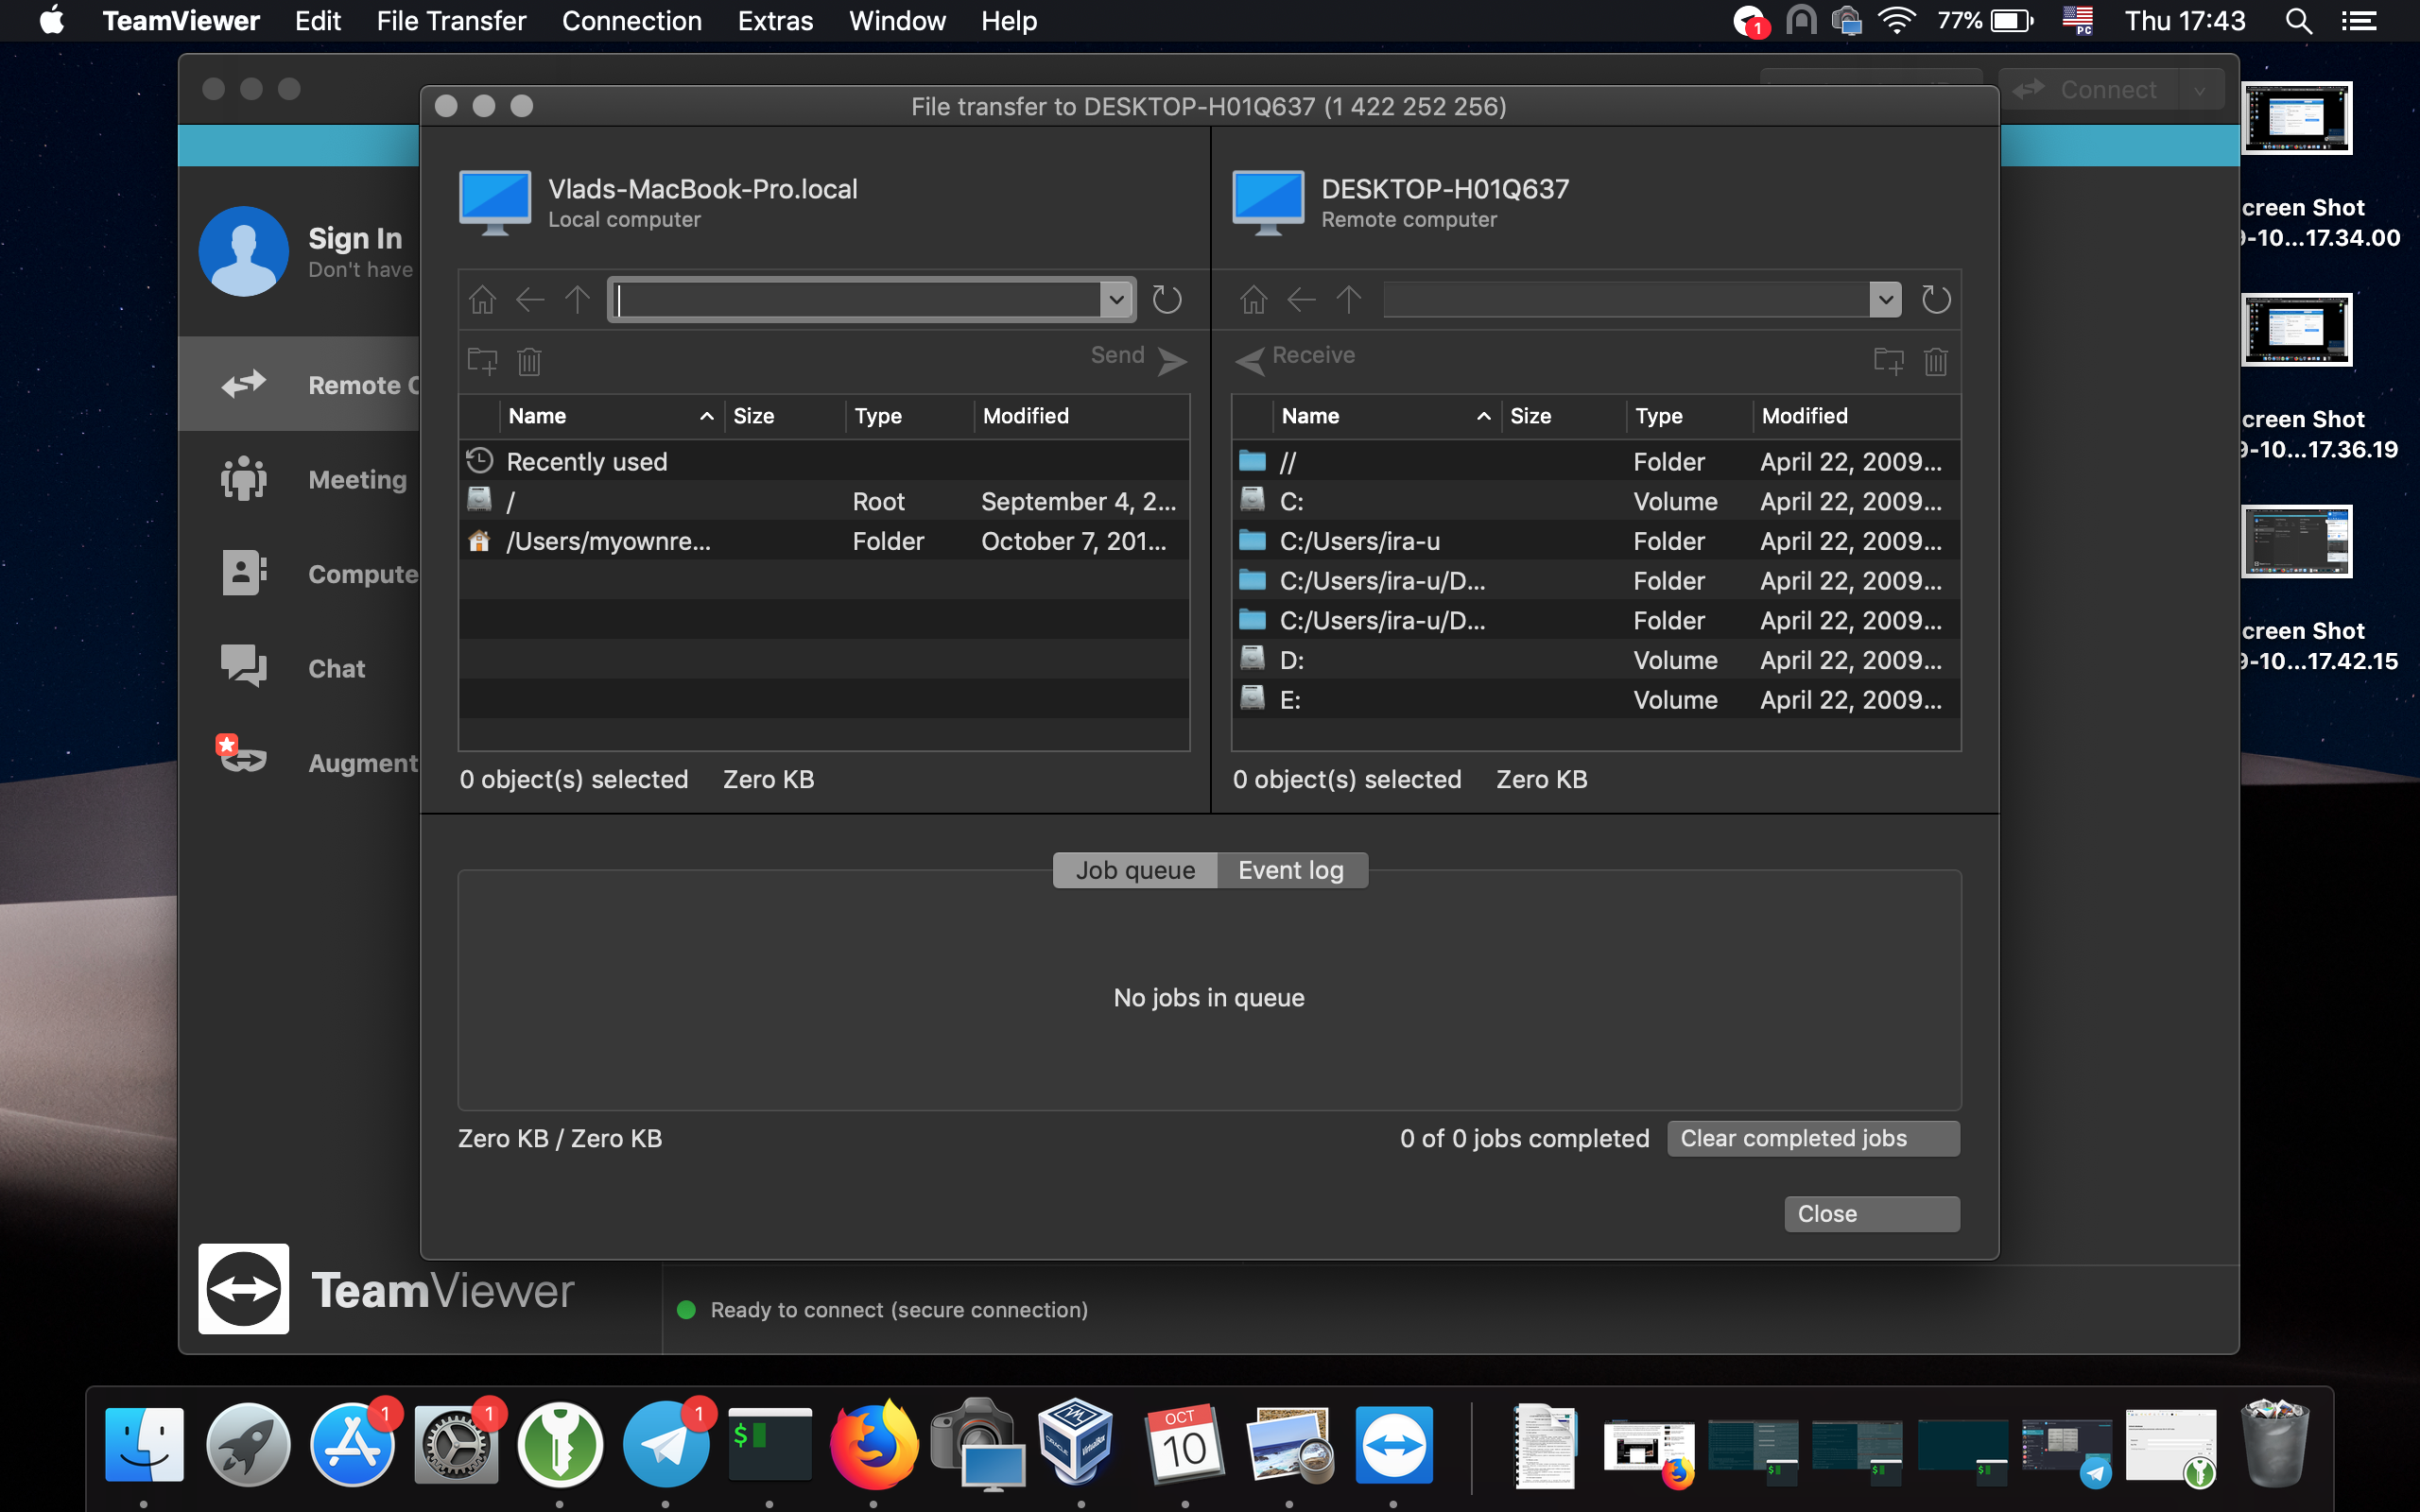
\includegraphics[width = \columnwidth]{./assets/p03-04.png}
					\caption{}
					\label{subfig:03-teamviewer-file-transfer-01}
				\end{subfigure}
				\begin{subfigure}[b]{8\gridunitwidth}
					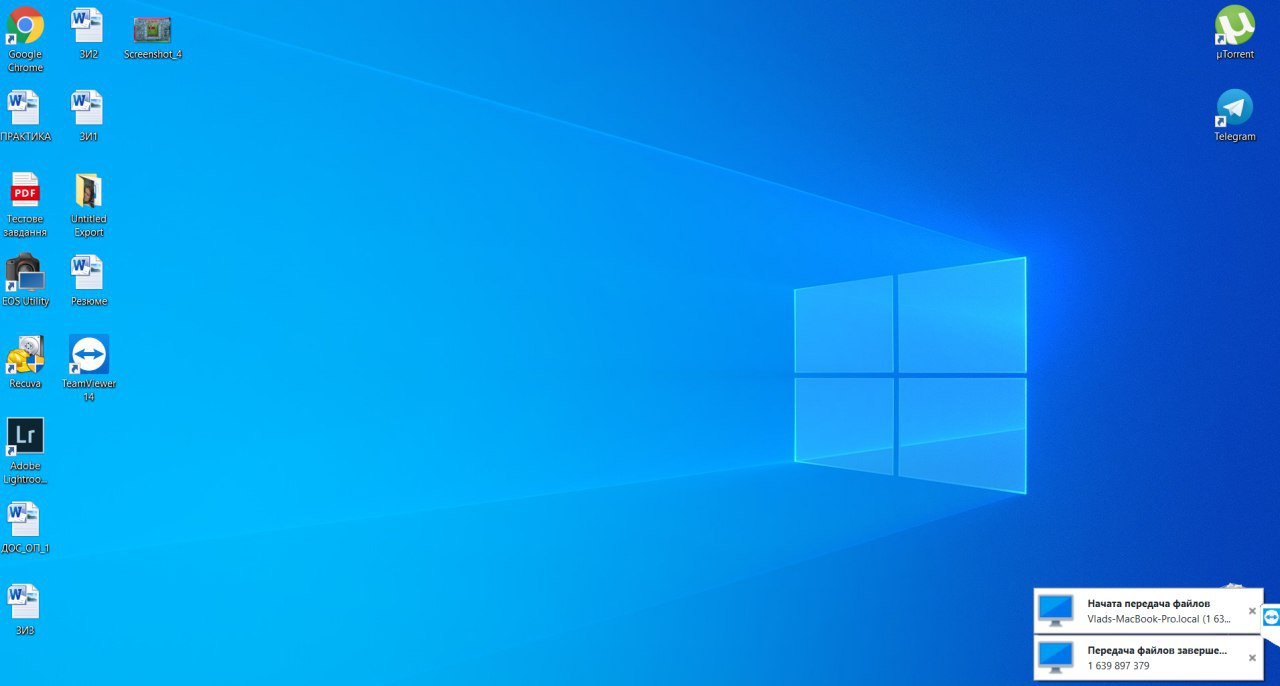
\includegraphics[width = \columnwidth]{./assets/p03-05.jpeg}
					\caption{}
					\label{subfig:03-teamviewer-file-transfer-02}
				\end{subfigure}
				\caption{Режим передачі файлів в~\textenglish{Teamviewer}: \subref{subfig:03-teamviewer-file-transfer-01}~— екран керуючої системи після початку передачі файлів, \subref{subfig:03-teamviewer-file-transfer-02}~— повідомлення про~початок передачі файлів}
				\label{fig:03-teamviewer-file-transfer}
			\end{figure}

			Режим~\textenglish{\allcaps{VPN}} надається виключно у~комерційній версії~\textenglish{Teamviewer}, тому ми~не~можемо випробувати його у~лабораторній роботі. Отже, ми~ознайомились із~функціональністю програми для~віддаленого керування~\textenglish{Teamviewer}.

		\subsection{Програма~\textenglish{Tight\allcaps{VNC}}}
			Встановлюємо програму~\textenglish{Tight\allcaps{VNC}} на~двох системах. На~керуючій системі запускаємо програму~\textenglish{Tight\allcaps{VNC}} як~додаток~(рис.~\ref{fig:04-tightvnc-01}).

			\begin{figure}[!htbp]
				\centering
				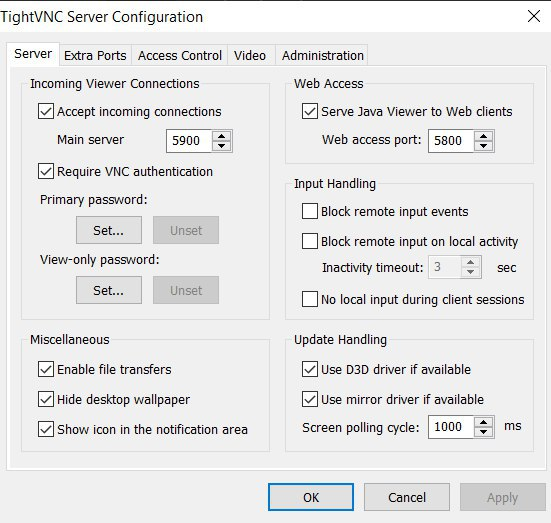
\includegraphics[height = 10\baselineskip]{./assets/p07-01.jpeg}
				\caption{Вікно додатку~\textenglish{Tight\allcaps{VNC}}}
				\label{fig:04-tightvnc-01}
			\end{figure}

			Після запуску сервера підключаємось до~нього за~допомогою~\textenglish{Tight\allcaps{VNC} Viewer}~(рис.~\ref{fig:04-tightvnc-01}). Таким чином ми~підключили клієнт до~сервера за~допомогою клієнта.

			\begin{figure}[!htbp]
				\centering
				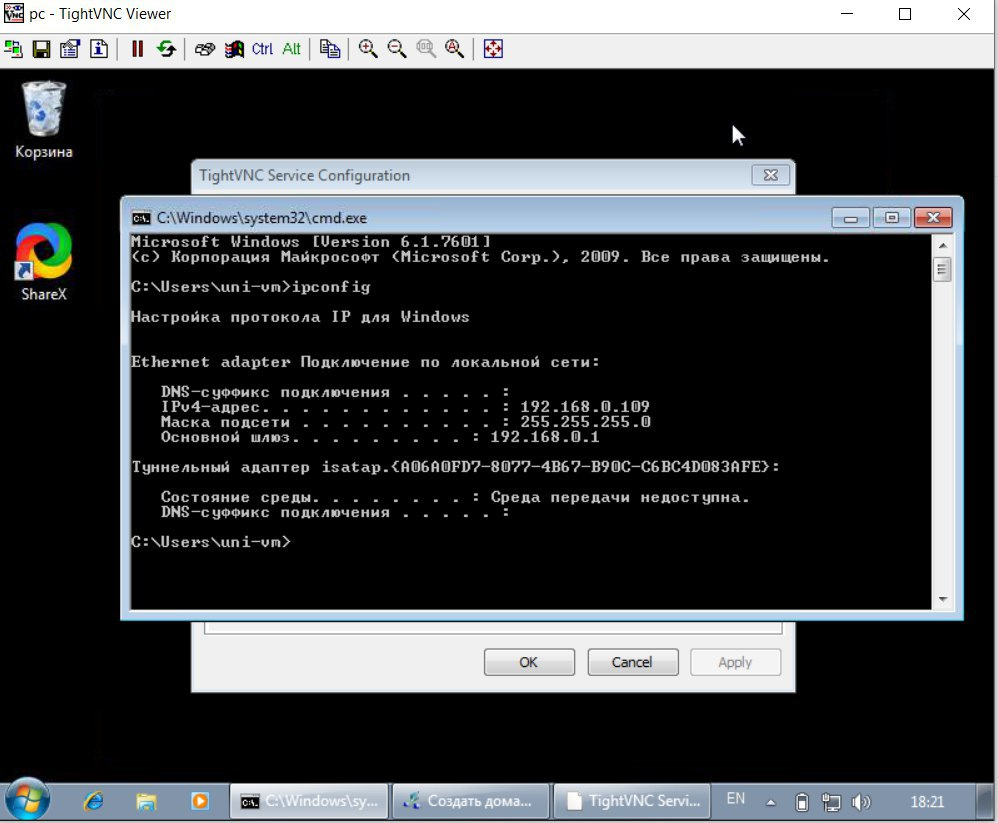
\includegraphics[height = 10\baselineskip]{./assets/p07-02.jpeg}
				\caption{Вікно додатку~\textenglish{Tight\allcaps{VNC} Viewer}}
				\label{fig:04-tightvnc-02}
			\end{figure}

			Далі ознайомимось з~роботою~\textenglish{Tight\allcaps{VNC} Viewer} в~режимі прослуховування. Для~цього на~першій системі увімкнемо цей~режим~(рис.~\ref{fig:04-tightvnc-03}), а~на~другій використаємо запущений~\textenglish{Tight\allcaps{VNC} Server}, щоб~підключити~\textenglish{Tight\allcaps{VNC} Viewer} першої системи у~режимі прослуховування до~другої системи. Таким чином ми~виконали зворотне з'єднання: підключення клієнта до~сервера за~допомогою сервера. Тепер спробуємо провести віддалене оновлення сервера програми~\textenglish{Tight\allcaps{VNC} Viewer}~(рис.~\ref{fig:04-tightvnc-04}).

			\begin{figure}[!htbp]
				\centering
				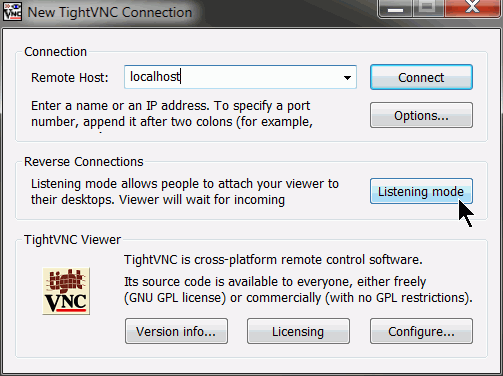
\includegraphics[height = 12\baselineskip]{./assets/p09-01.png}
				\caption{Вікно для~увімкнення режиму прослуховування~\textenglish{Tight\allcaps{VNC}}}
				\label{fig:04-tightvnc-03}
			\end{figure}

			\begin{figure}[!htbp]
				\centering
				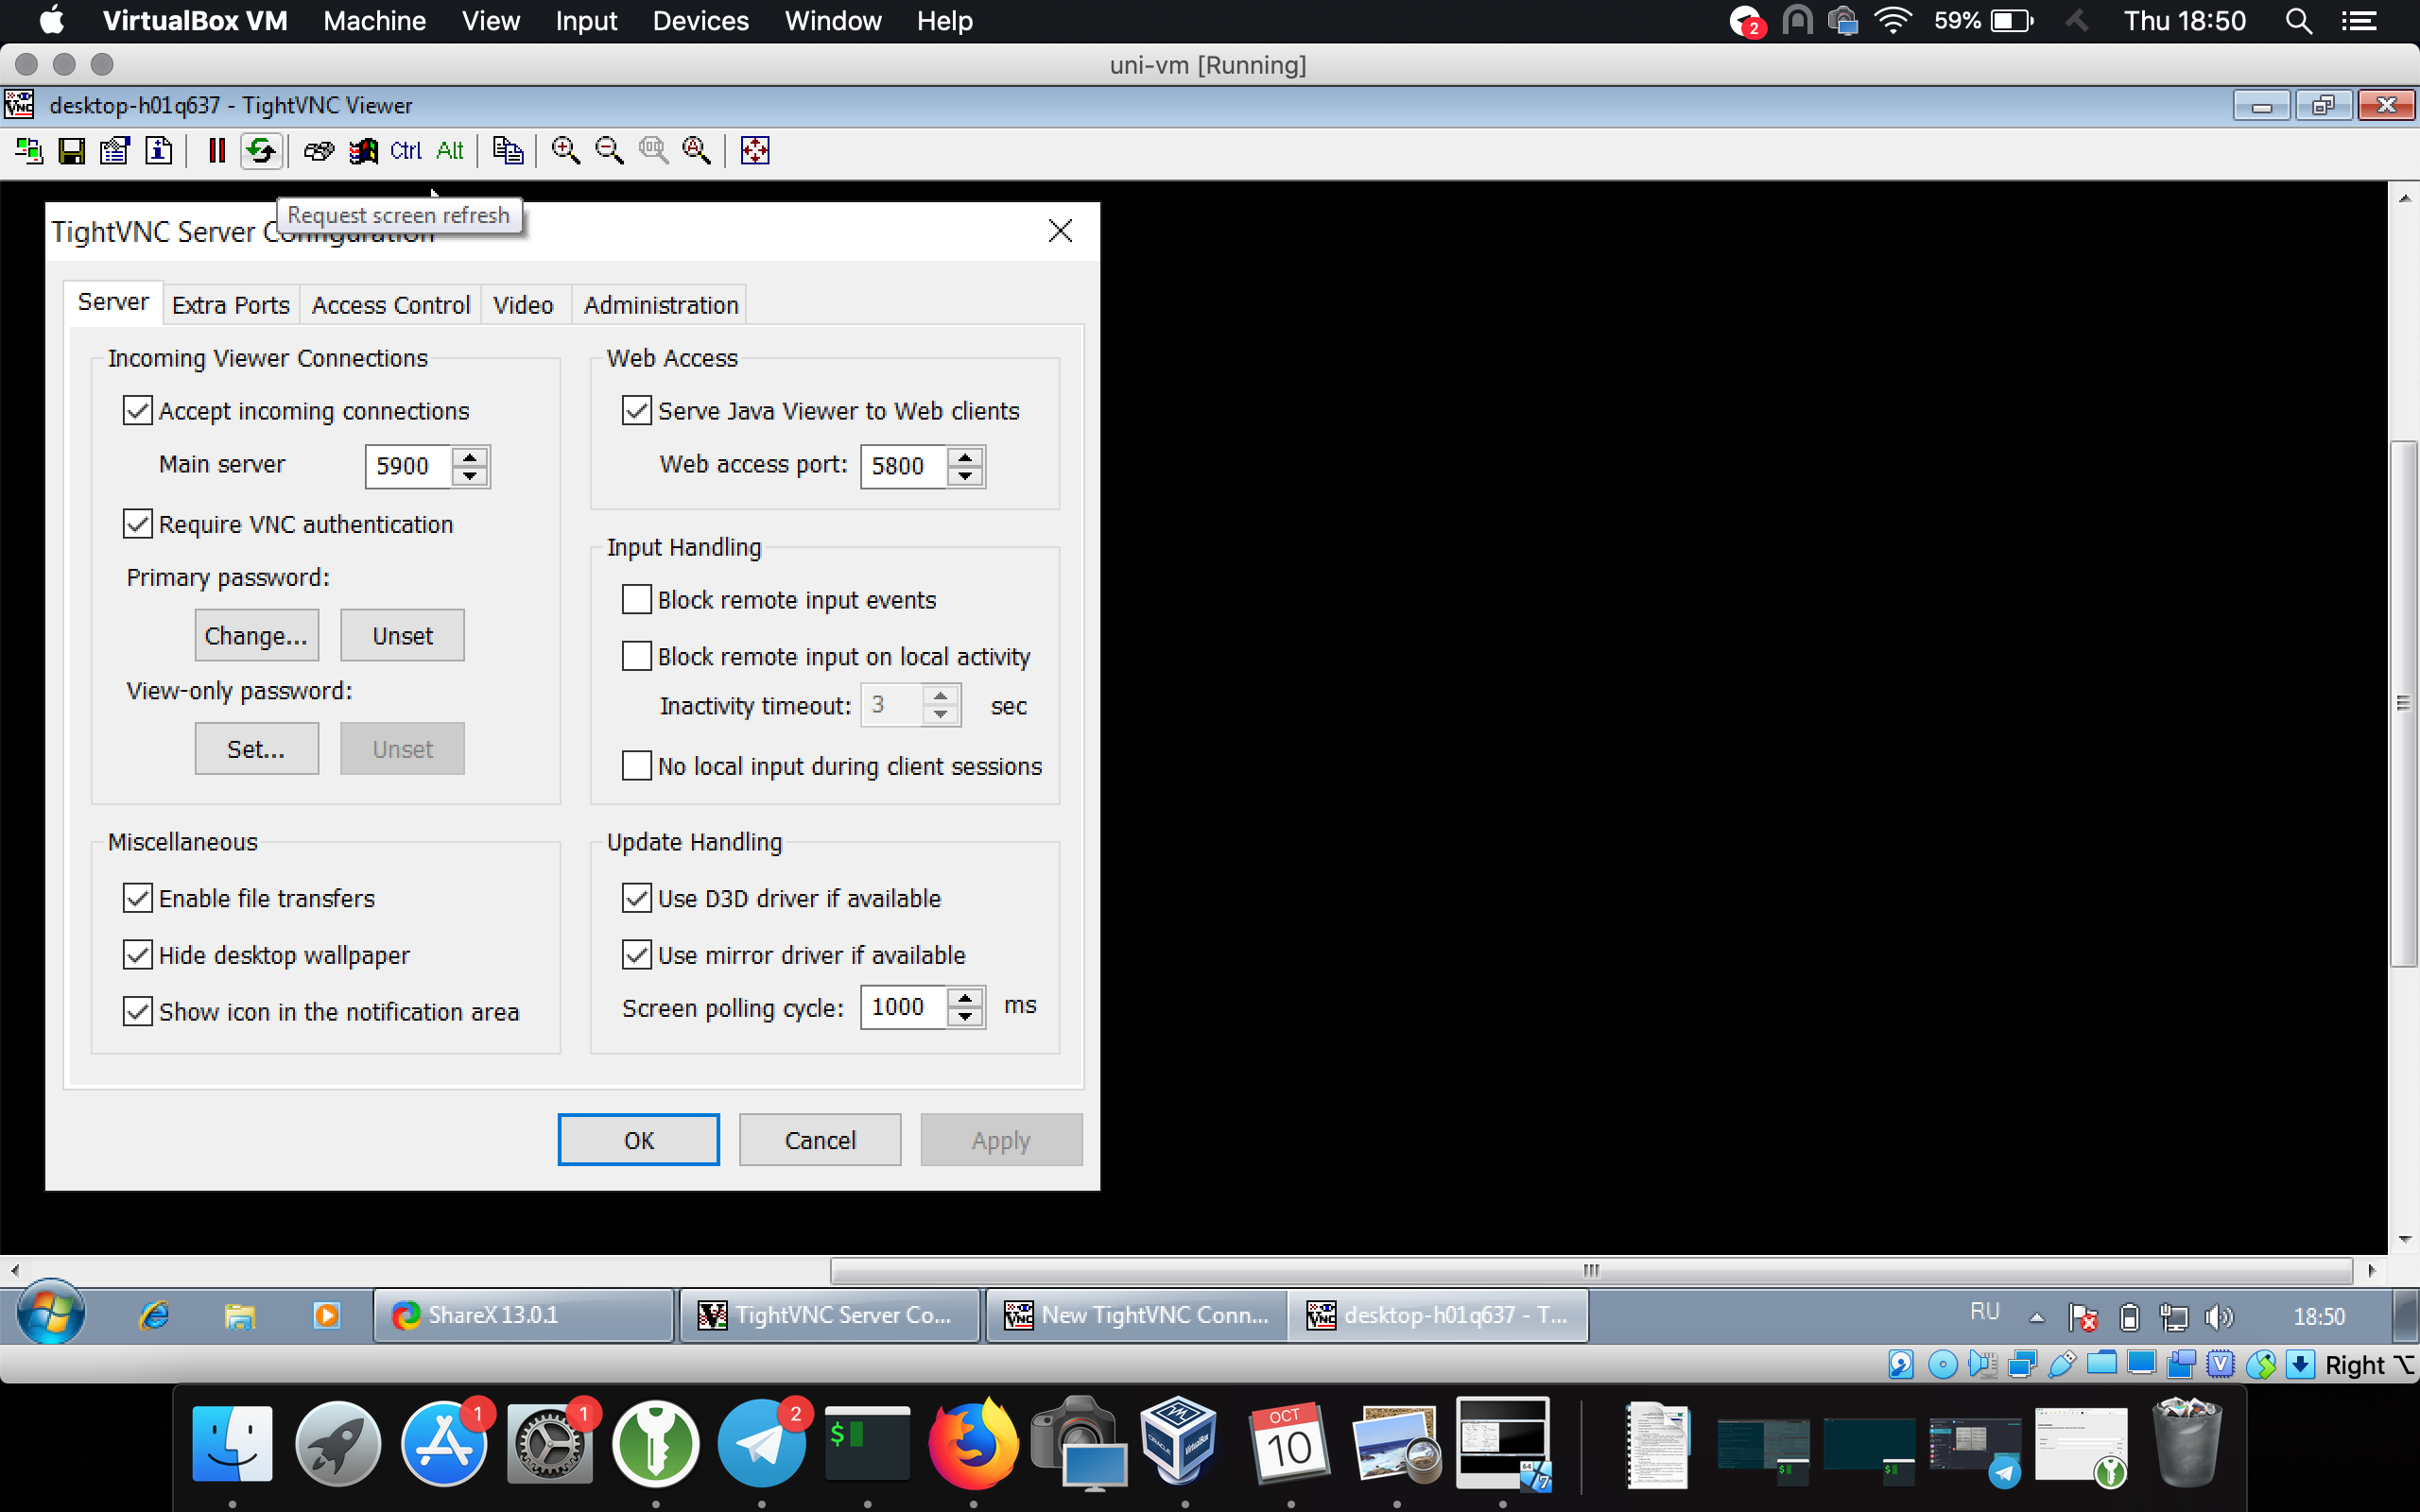
\includegraphics[height = 12\baselineskip]{./assets/p11-01.png}
				\caption{Підключення до~\textenglish{Tight\allcaps{VNC} Viewer} у~режимі прослуховування і~подальше віддалене оновлення сервера~\textenglish{Tight\allcaps{VNC}}}
				\label{fig:04-tightvnc-04}
			\end{figure}

			Запустимо~\textenglish{Tight\allcaps{VNC}} як~службу, виконаємо доступні команди і~зафіксуємо результати. Наприклад, такими командами є~передача файлів~(рис.~\ref{subfig:04-tightvnc-05-01}), зміна масштабу віртуального робочого столу~(рис.~\ref{subfig:04-tightvnc-05-02}, \ref{subfig:04-tightvnc-05-03}).

			\begin{figure}[!htbp]
				\centering
				\begin{subfigure}[b]{\columnwidth}
					\centering
					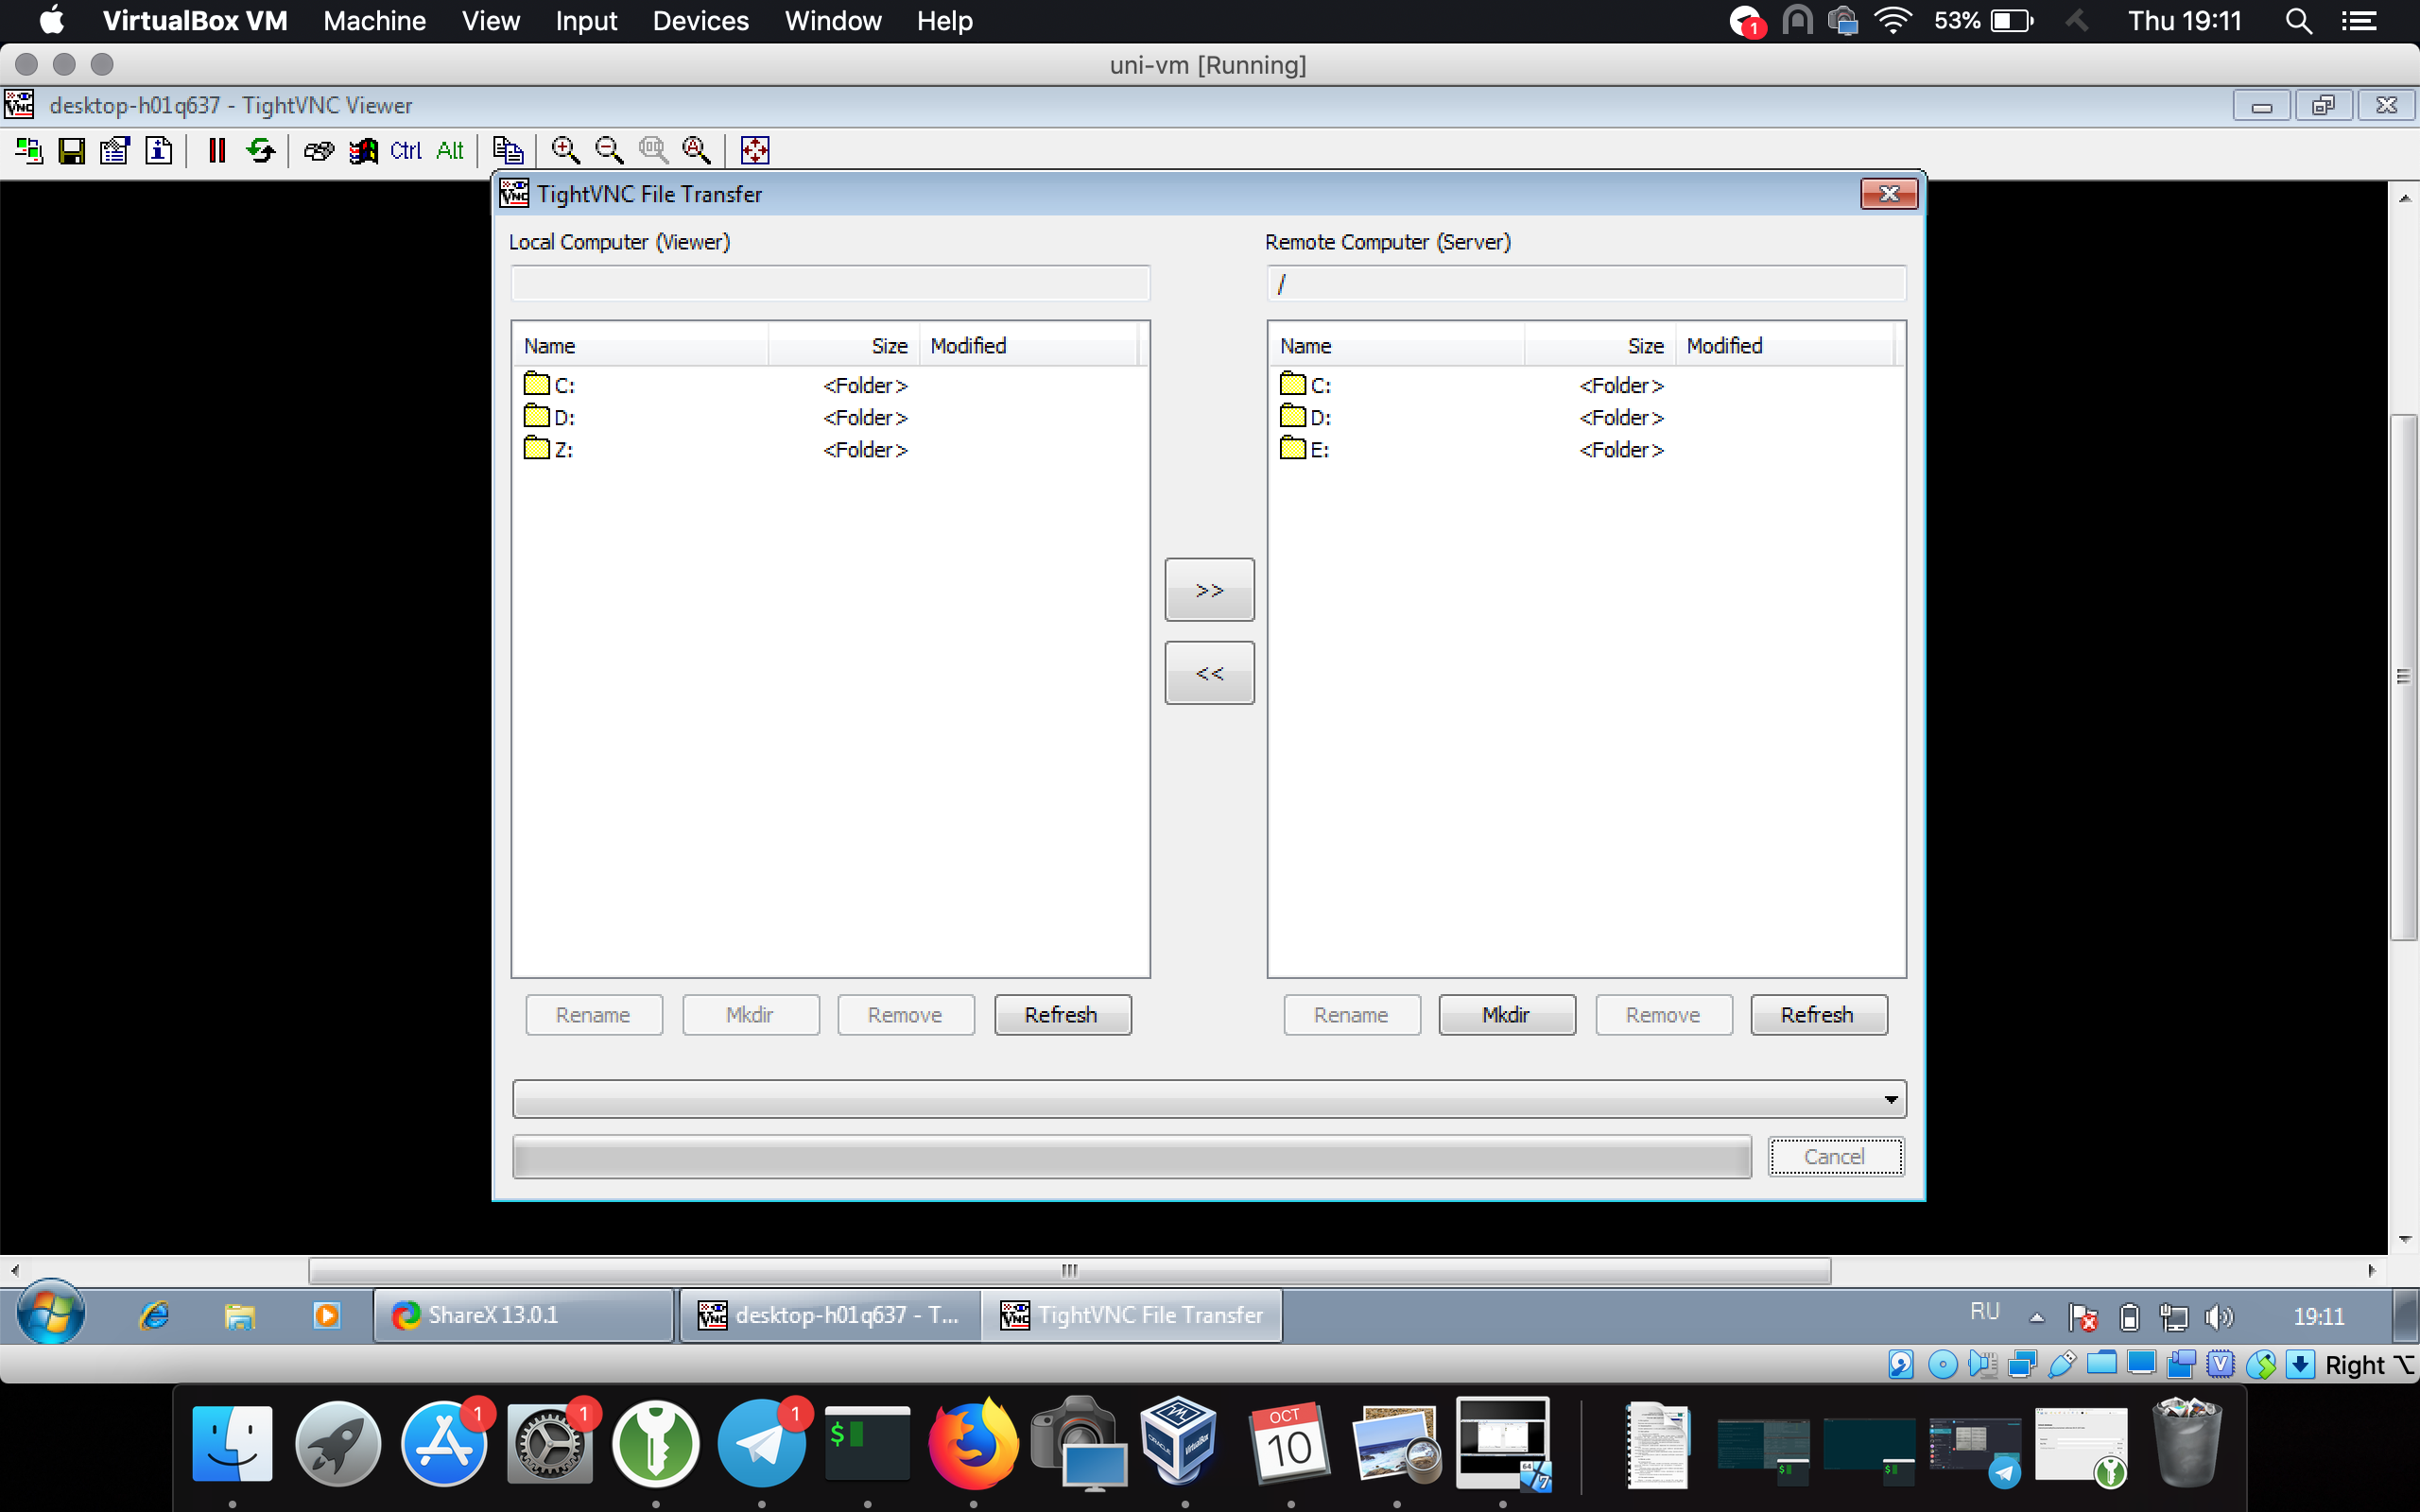
\includegraphics[height = 10\baselineskip]{./assets/p13-01.png}
					\caption{}
					\label{subfig:04-tightvnc-05-01}
				\end{subfigure}
				\begin{subfigure}[b]{\columnwidth}
					\centering
					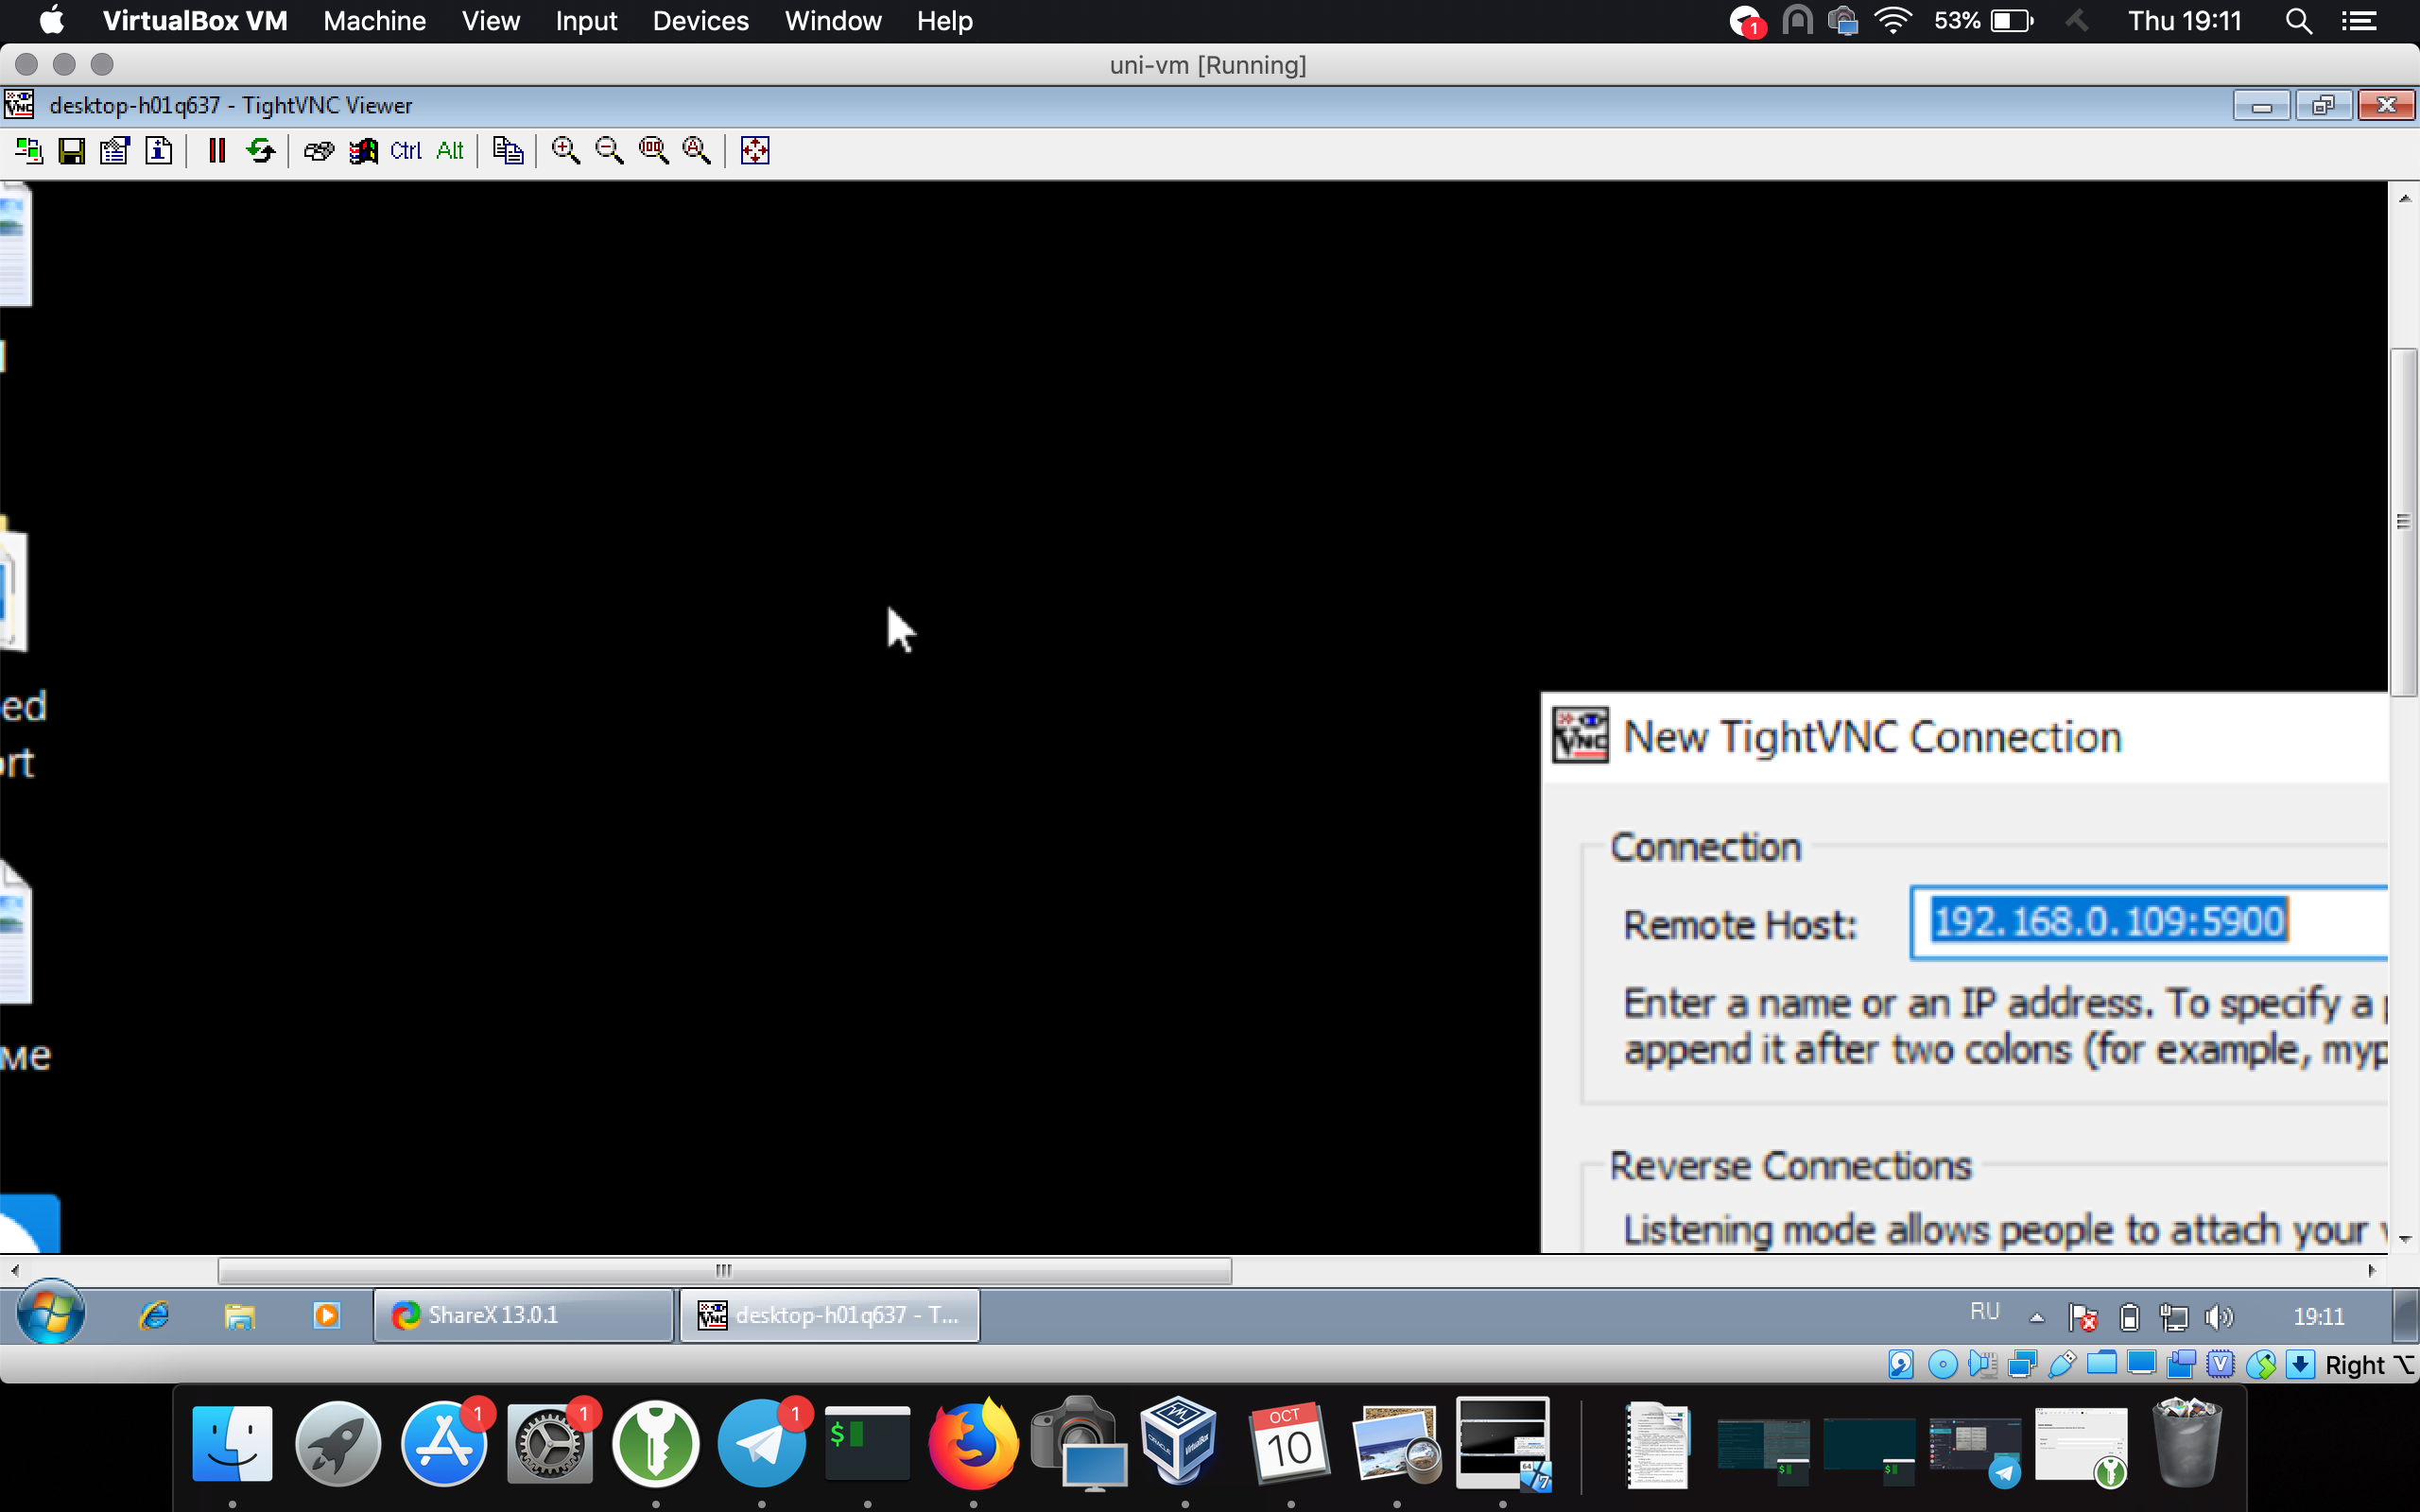
\includegraphics[height = 10\baselineskip]{./assets/p13-02.png}
					\caption{}
					\label{subfig:04-tightvnc-05-02}
				\end{subfigure}
				\begin{subfigure}[b]{\columnwidth}
					\centering
					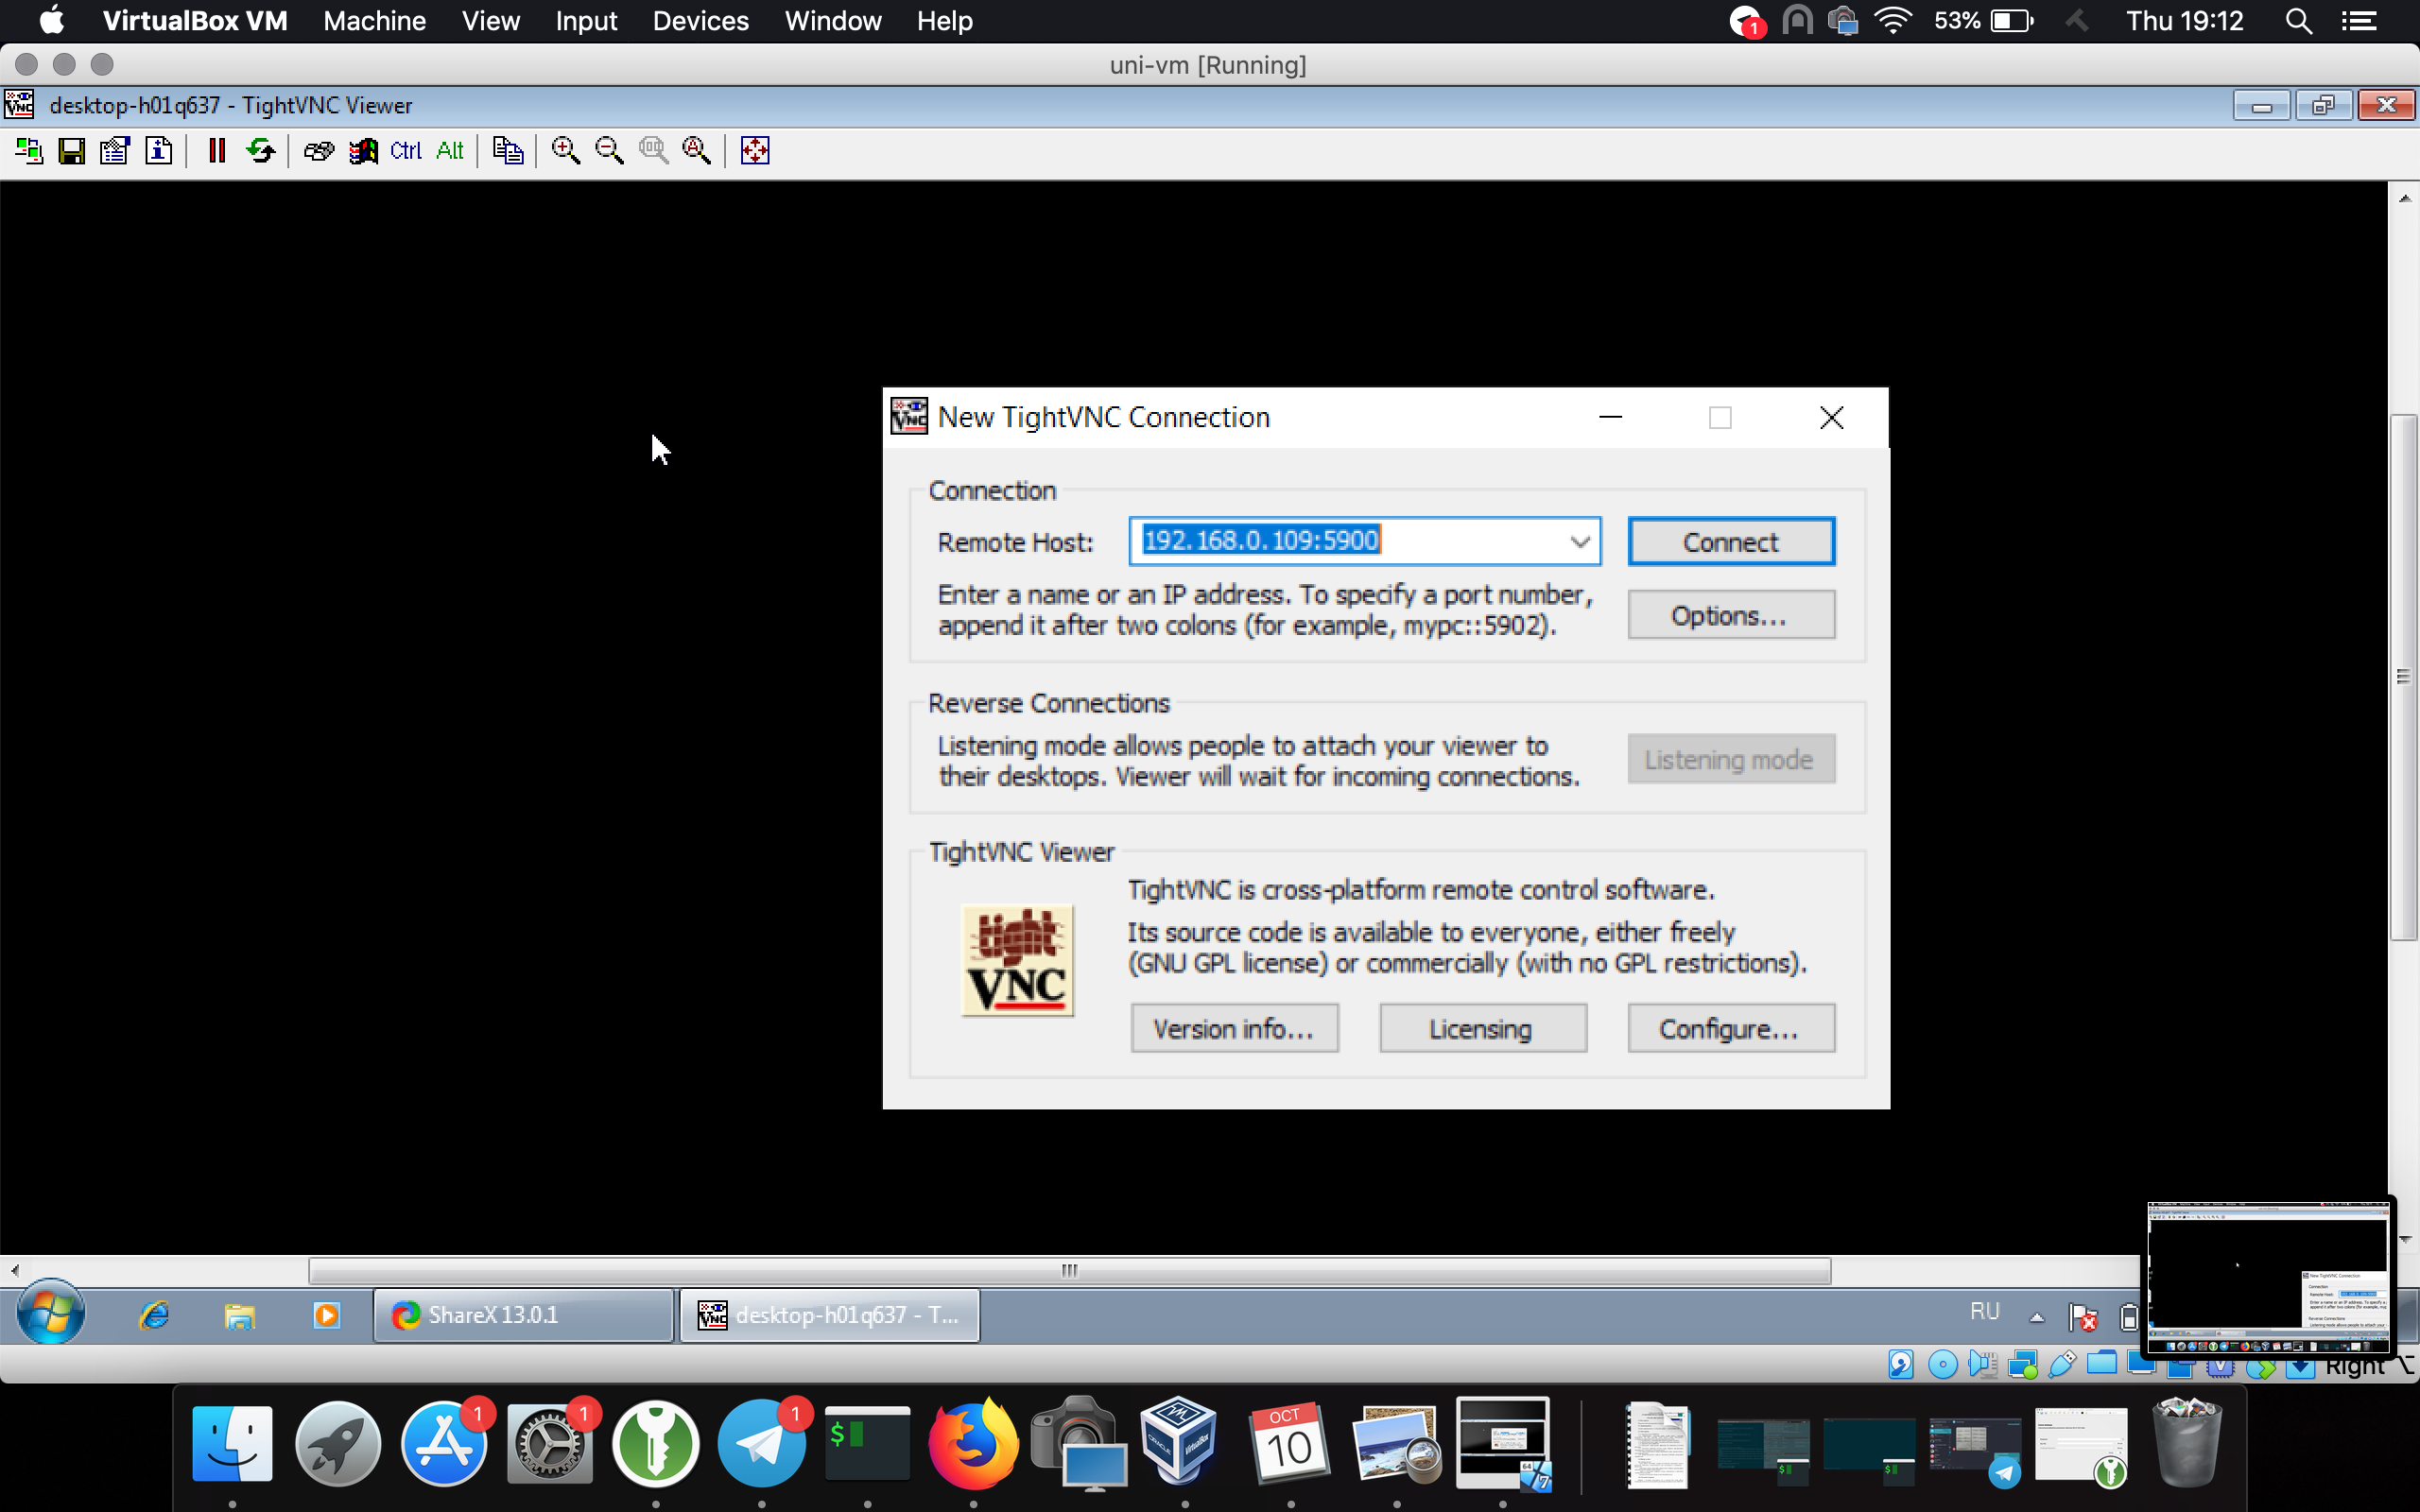
\includegraphics[height = 10\baselineskip]{./assets/p13-03.png}
					\caption{}
					\label{subfig:04-tightvnc-05-03}
				\end{subfigure}
				\caption{Виконання команд в~\textenglish{Tight\allcaps{VNC}}: \subref{subfig:04-tightvnc-05-01}~— передача файлів, \subref{subfig:04-tightvnc-05-02}, \subref{subfig:04-tightvnc-05-03}~— зміна масштабу віртуального робочого столу}
				\label{fig:04-tightvnc-05}
			\end{figure}

			Спробуємо використати веб-браузер як~переглядач віддаленого робочого столу~\textenglish{Tight\allcaps{VNC}}. Для~цього переконуємось, що~в~системі, яка~буде підключатись до~віддаленого робочого столу, встановлено середовище~\textenglish{Java Runtime Environment}, а~також що~увімкнена опція~«Надавати веб-клієнтам доступ до~\textenglish{Java Viewer}». Далі відкриваємо веб-браузер за~адресою веб-сервера~\textenglish{Tight\allcaps{VNC}} і~спостерігаємо результат~(рис.~\ref{fig:04-tightvnc-06}).

			\begin{figure}[!htbp]
				\centering
				\begin{subfigure}[b]{4 \gridunitwidth - 0.5em}
					\centering
					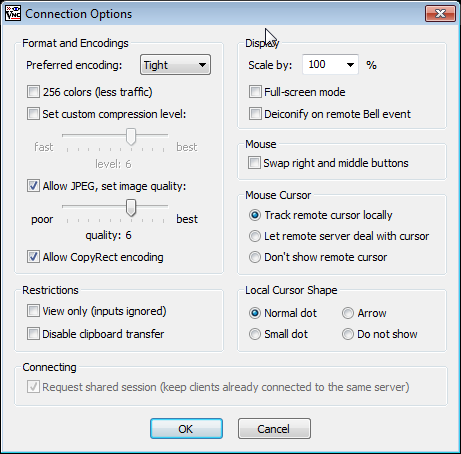
\includegraphics[width = \columnwidth]{./assets/p14-01.png}
					\caption{}
					\label{subfig:04-tightvnc-06-01}
				\end{subfigure}%
				\hspace{1em}%
				\begin{subfigure}[b]{8 \gridunitwidth - 0.5em}
					\centering
					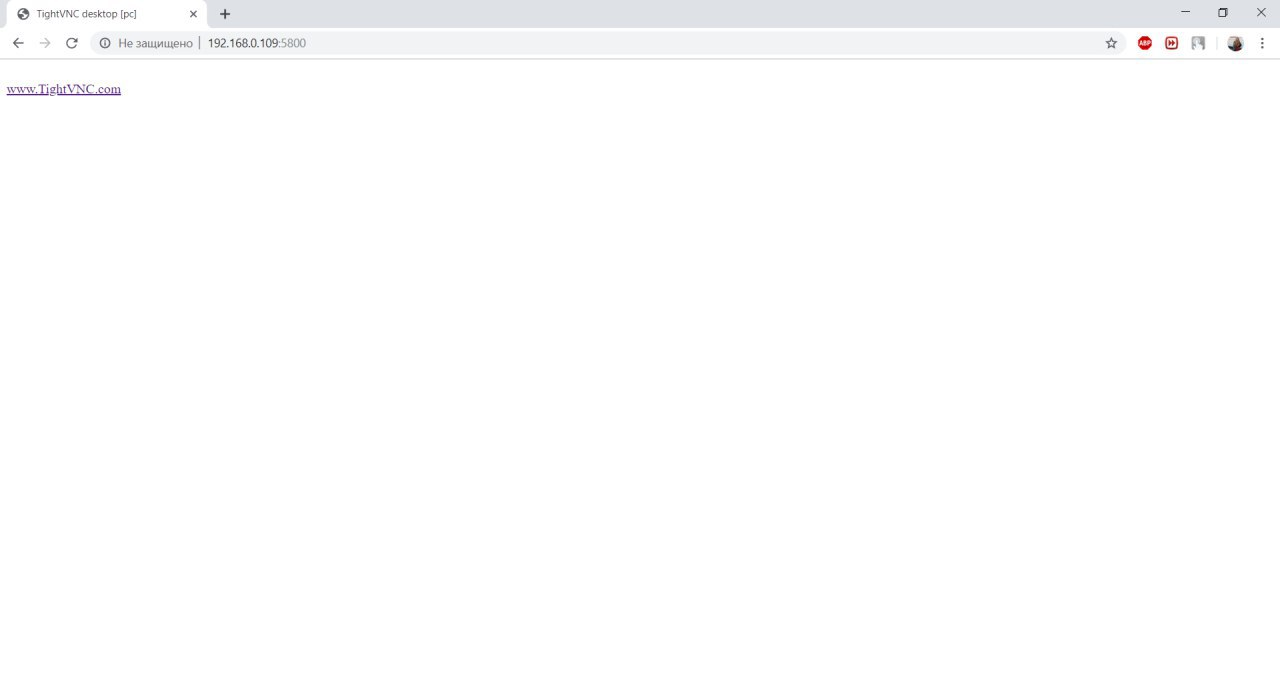
\includegraphics[width = \columnwidth]{./assets/p14-02.jpeg}
					\caption{}
					\label{subfig:04-tightvnc-06-02}
				\end{subfigure}
				\caption{Спроба підключитись до~сервера~\textenglish{Tight\allcaps{VNC}} через веб-браузер: \subref{subfig:04-tightvnc-06-01}~— налаштування сервера, \subref{subfig:04-tightvnc-06-02}~— відкрита веб-сторінка}
				\label{fig:04-tightvnc-06}
			\end{figure}

			В~результаті бачимо, що~\textenglish{Tight\allcaps{VNC}} не~повертає~\textenglish{Java}-аплет, і~тому неможливо підключитись до~віддаленого робочого столу за~допомогою веб-браузера.

		\subsection{Програма \textenglish{Radmin}}
			Встановлюємо програму~\textenglish{Radmin Server} на~керованій системі та~\textenglish{Radmin Viewer}~— на~керуючій. Запускаємо~\textenglish{Radmin Server} на~керованій машині та~додаємо користувача. Для~цього заходимо у~налаштування і~натискаємо на~кнопку~«Додати користувача», а~потім надаємо йому всі~необхідні права. В~результаті був~створений користувач, якій може підключитись до~сервера~(рис.~\ref{fig:05-radmin-01}).

			\begin{figure}[!htbp]
				\centering
				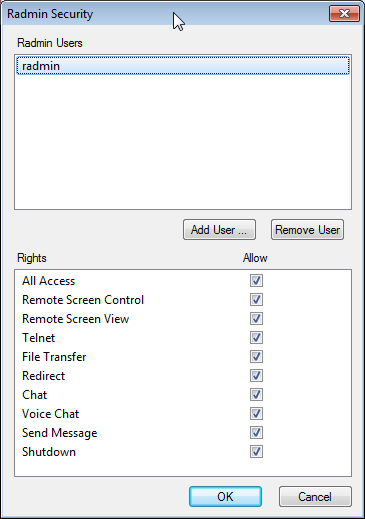
\includegraphics[height = 10\baselineskip]{./assets/p16-01.png}
				\caption{Вікно додавання користувачів~\textenglish{Radmin Server}}
				\label{fig:05-radmin-01}
			\end{figure}

			Створивши користувача на~керованій системі, переходимо до~керуючої системи. Спочатку запускаємо~\textenglish{Radmin Viewer} на~керуючій машині та~додаємо віддалений комп'ютер~(рис.~\ref{subfig:05-radmin-02-01}), а~потім підключаємось до~віддаленого комп'ютера~(рис.~\ref{subfig:05-radmin-02-02}).

			\begin{figure}[!htbp]
				\centering
				\begin{subfigure}{0.5\columnwidth - 0.5em}
					\centering
					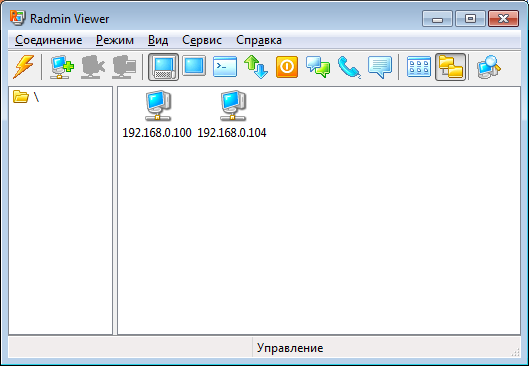
\includegraphics[width = \columnwidth]{./assets/p16-02.png}
					\caption{}
					\label{subfig:05-radmin-02-01}
				\end{subfigure}%
				\hspace{1em}%
				\begin{subfigure}{0.5\columnwidth - 0.5em}
					\centering
					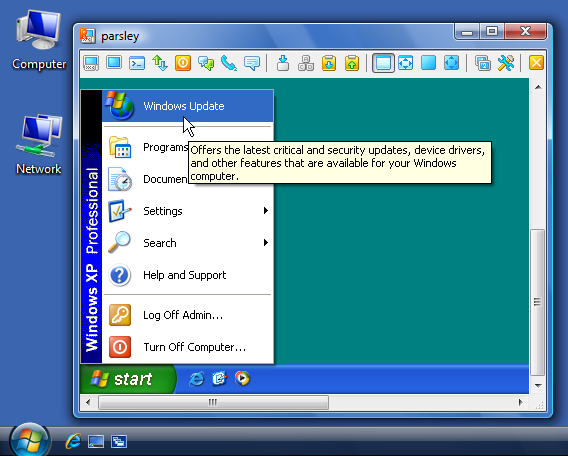
\includegraphics[width = \columnwidth]{./assets/p16-03.png}
					\caption{}
					\label{subfig:05-radmin-02-02}
				\end{subfigure}
				\caption{Підключення до~керованої системи: \subref{subfig:05-radmin-02-01}~— вікно~\textenglish{Radmin Viewer} після створення двох віддалених комп'ютерів, \subref{subfig:05-radmin-02-02}~— вікно~\textenglish{Radmin Viewer} після підключення до~віддаленого комп'ютера}
				\label{fig:05-radmin-02}
			\end{figure}

			Отже, ми~ознайомились з~комплектом програм для~віддаленого керування комп'ютерами~\textenglish{Radmin}.

	\section{Висновок}
		Виконуючи дану лабораторну роботу, ми~ознайомились із~програмними засобами віддаленого адміністрування та~відповідними протоколами, а~також встановили програми віддаленого адміністрування і~навчились їх~використовувати.

\end{document}
